%==============================================================================
% tento soubor pouzijte jako zaklad
% this file should be used as a base for the thesis
% Autoři / Authors: 2008 Michal Bidlo, 2018 Jaroslav Dytrych
% Kontakt pro dotazy a připomínky: dytrych@fit.vutbr.cz
% Contact for questions and comments: dytrych@fit.vutbr.cz
%==============================================================================
% kodovani: UTF-8 (zmena prikazem iconv, recode nebo cstocs)
% encoding: UTF-8 (you can change it by command iconv, recode or cstocs)
%------------------------------------------------------------------------------
% zpracování / processing: make, make pdf, make clean
%==============================================================================
% Soubory, které je nutné upravit: / Files which have to be edited:
%   projekt-20-literatura-bibliography.bib - literatura / bibliography
%   projekt-01-kapitoly-chapters.tex - obsah práce / the thesis content
%   projekt-30-prilohy-appendices.tex - přílohy / appendices
%==============================================================================

\documentclass[english]{fitthesis} % bez zadání - pro začátek práce, aby nebyl problém s překladem
%\documentclass[english]{fitthesis} % without assignment - for the work start to avoid compilation problem
%\documentclass[zadani]{fitthesis} % odevzdani do wisu a/nebo tisk s barevnými odkazy - odkazy jsou barevné
%\documentclass[english,zadani]{fitthesis} % for submission to the IS FIT and/or print with color links - links are color
%\documentclass[zadani,print]{fitthesis} % pro černobílý tisk - odkazy jsou černé
%\documentclass[english,zadani,print]{fitthesis} % for the black and white print - links are black
%\documentclass[zadani,cprint]{fitthesis} % pro barevný tisk - odkazy jsou černé, znak VUT barevný
%\documentclass[english,zadani,cprint]{fitthesis} % for the print - links are black, logo is color
% * Je-li práce psaná v anglickém jazyce, je zapotřebí u třídy použít 
%   parametr english následovně:
%   If thesis is written in english, it is necessary to use 
%   parameter english as follows:
%      \documentclass[english]{fitthesis}
% * Je-li práce psaná ve slovenském jazyce, je zapotřebí u třídy použít 
%   parametr slovak následovně:
%   If the work is written in the Slovak language, it is necessary 
%   to use parameter slovak as follows:
%      \documentclass[slovak]{fitthesis}
% * Je-li práce psaná v anglickém jazyce se slovenským abstraktem apod., 
%   je zapotřebí u třídy použít parametry english a enslovak následovně:
%   If the work is written in English with the Slovak abstract, etc., 
%   it is necessary to use parameters english and enslovak as follows:
%      \documentclass[english,enslovak]{fitthesis}

% Základní balíčky jsou dole v souboru šablony fitthesis.cls
% Basic packages are at the bottom of template file fitthesis.cls
% zde můžeme vložit vlastní balíčky / you can place own packages here

% Kompilace po částech (rychlejší, ale v náhledu nemusí být vše aktuální)
% Compilation piecewise (faster, but not all parts in preview will be up-to-date)
% \usepackage{subfiles}

% Nastavení cesty k obrázkům
% Setting of a path to the pictures
%\graphicspath{{obrazky-figures/}{./obrazky-figures/}}
%\graphicspath{{obrazky-figures/}{../obrazky-figures/}}

%---rm---------------
\renewcommand{\rmdefault}{lmr}%zavede Latin Modern Roman jako rm / set Latin Modern Roman as rm
%---sf---------------
\renewcommand{\sfdefault}{qhv}%zavede TeX Gyre Heros jako sf
%---tt------------
\renewcommand{\ttdefault}{lmtt}% zavede Latin Modern tt jako tt





% vypne funkci šablony, která automaticky nahrazuje uvozovky,
% aby nebyly prováděny nevhodné náhrady v popisech API apod.
% disables function of the template which replaces quotation marks
% to avoid unnecessary replacements in the API descriptions etc.
\csdoublequotesoff



\usepackage[outputdir=out]{minted}
\usepackage{caption}
\usepackage{graphicx}
\usepackage{grffile}
\usepackage{listings, listings-rust}

\usepackage{tikz}
\usepackage{tikz-uml}

\lstdefinestyle{freefempp}{
language=Rust,
basicstyle=\footnotesize\ttfamily,
commentstyle=\itshape\color{violet},
% float,
frame=single,
numbers=left
}

\lstset{style=freefempp}

\lstnewenvironment{code}[1][]%
{\noindent\minipage{\linewidth}\medskip
\lstset{basicstyle=\ttfamily\footnotesize,frame=single,#1}}
{\endminipage}

% =======================================================================
% balíček "hyperref" vytváří klikací odkazy v pdf, pokud tedy použijeme pdflatex
% problém je, že balíček hyperref musí být uveden jako poslední, takže nemůže
% být v šabloně
% "hyperref" package create clickable links in pdf if you are using pdflatex.
% Problem is that this package have to be introduced as the last one so it 
% can not be placed in the template file.
\ifWis
\ifx\pdfoutput\undefined % nejedeme pod pdflatexem / we are not using pdflatex
\else
  \usepackage{color}
  \usepackage[unicode,colorlinks,hyperindex,plainpages=false,pdftex]{hyperref}
  \definecolor{hrcolor-ref}{RGB}{223,52,30}
  \definecolor{hrcolor-cite}{HTML}{2F8F00}
  \definecolor{hrcolor-urls}{HTML}{092EAB}
  \hypersetup{
	linkcolor=hrcolor-ref,
	citecolor=hrcolor-cite,
	filecolor=magenta,
	urlcolor=hrcolor-urls
  }
  \def\pdfBorderAttrs{/Border [0 0 0] }  % bez okrajů kolem odkazů / without margins around links
  \pdfcompresslevel=9
\fi
\else % pro tisk budou odkazy, na které se dá klikat, černé / for the print clickable links will be black
\ifx\pdfoutput\undefined % nejedeme pod pdflatexem / we are not using pdflatex
\else
  \usepackage{color}
  \usepackage[unicode,colorlinks,hyperindex,plainpages=false,pdftex,urlcolor=black,linkcolor=black,citecolor=black]{hyperref}
  \definecolor{links}{rgb}{0,0,0}
  \definecolor{anchors}{rgb}{0,0,0}
  \def\AnchorColor{anchors}
  \def\LinkColor{links}
  \def\pdfBorderAttrs{/Border [0 0 0] } % bez okrajů kolem odkazů / without margins around links
  \pdfcompresslevel=9
\fi
\fi
% Řešení problému, kdy klikací odkazy na obrázky vedou za obrázek
% This solves the problems with links which leads after the picture
\usepackage[all]{hypcap}

% Informace o práci/projektu / Information about the thesis
%---------------------------------------------------------------------------
\projectinfo{
  %Prace / Thesis
  project={SP},            %typ práce BP/SP/DP/DR  / thesis type (SP = term project)
  year={2018},             % rok odevzdání / year of submission
  date=\today,             % datum odevzdání / submission date
  %Nazev prace / thesis title
  title.cs={Návrh a implementace distribuovaného systému pro algoritmické obchodování},  % název práce v češtině či slovenštině (dle zadání) / thesis title in czech language (according to assignment)
  title.en={Design and Implementation of Distributed System for Algorithmic Trading}, % název práce v angličtině / thesis title in english
  %title.length={14.5cm}, % nastavení délky bloku s titulkem pro úpravu zalomení řádku (lze definovat zde nebo níže) / setting the length of a block with a thesis title for adjusting a line break (can be defined here or below)
  %Autor / Author
  author.name={Michal},   % jméno autora / author name
  author.surname={Hornický},   % příjmení autora / author surname
  author.title.p={Bc.}, % titul před jménem (nepovinné) / title before the name (optional)
  %author.title.a={Ph.D.}, % titul za jménem (nepovinné) / title after the name (optional)
  %Ustav / Department
  department={UIFS}, % doplňte příslušnou zkratku dle ústavu na zadání: UPSY/UIFS/UITS/UPGM / fill in appropriate abbreviation of the department according to assignment: UPSY/UIFS/UITS/UPGM
  % Školitel / supervisor
  supervisor.name={Marek},   % jméno školitele / supervisor name
  supervisor.surname={Rychlý},   % příjmení školitele / supervisor surname
  supervisor.title.p={RNDr.},   %titul před jménem (nepovinné) / title before the name (optional)
  supervisor.title.a={Ph.D.},    %titul za jménem (nepovinné) / title after the name (optional)
  % Klíčová slova / keywords
  keywords.cs={TODO}, % klíčová slova v českém či slovenském jazyce / keywords in czech or slovak language
  keywords.en={Trading, Algorithmic trading, Cloud, Distributed system, Rust, Kubernetes, }, % klíčová slova v anglickém jazyce / keywords in english
  %keywords.en={Here, individual keywords separated by commas will be written in English.},
  % Abstrakt / Abstract
  abstract.cs={Do tohoto odstavce bude zapsán výtah (abstrakt) práce v českém (slovenském) jazyce.}, % abstrakt v českém či slovenském jazyce / abstract in czech or slovak language
  abstract.en={Do tohoto odstavce bude zapsán výtah (abstrakt) práce v anglickém jazyce.}, % abstrakt v anglickém jazyce / abstract in english
  %abstract.en={An abstract of the work in English will be written in this paragraph.},
  % Prohlášení (u anglicky psané práce anglicky, u slovensky psané práce slovensky) / Declaration (for thesis in english should be in english)
  declaration={Prohlašuji, že jsem tuto bakalářskou práci vypracoval samostatně pod vedením pana X...
Další informace mi poskytli...
Uvedl jsem všechny literární prameny a publikace, ze kterých jsem čerpal.},
  %declaration={Hereby I declare that this bachelor's thesis was prepared as an original author’s work under the supervision of Mr. X
% The supplementary information was provided by Mr. Y
% All the relevant information sources, which were used during preparation of this thesis, are properly cited and included in the list of references.},
  % Poděkování (nepovinné, nejlépe v jazyce práce) / Acknowledgement (optional, ideally in the language of the thesis)
  acknowledgment={V této sekci je možno uvést poděkování vedoucímu práce a těm, kteří poskytli odbornou pomoc
(externí zadavatel, konzultant, apod.).},
  %acknowledgment={Here it is possible to express thanks to the supervisor and to the people which provided professional help
%(external submitter, consultant, etc.).},
  % Rozšířený abstrakt (cca 3 normostrany) - lze definovat zde nebo níže / Extended abstract (approximately 3 standard pages) - can be defined here or below
  %extendedabstract={Do tohoto odstavce bude zapsán rozšířený výtah (abstrakt) práce v českém (slovenském) jazyce.},
  %faculty={FIT}, % FIT/FEKT/FSI/FA/FCH/FP/FAST/FAVU/USI/DEF
  faculty.cs={Fakulta informačních technologií}, % Fakulta v češtině - pro využití této položky výše zvolte fakultu DEF / Faculty in Czech - for use of this entry select DEF above
  faculty.en={Faculty of Information Technology}, % Fakulta v angličtině - pro využití této položky výše zvolte fakultu DEF / Faculty in English - for use of this entry select DEF above
  %department.cs={Ústav matematiky}, % Ústav v češtině - pro využití této položky výše zvolte ústav DEF nebo jej zakomentujte / Department in Czech - for use of this entry select DEF above or comment it out
  %department.en={Institute of Mathematics} % Ústav v angličtině - pro využití této položky výše zvolte ústav DEF nebo jej zakomentujte / Department in English - for use of this entry select DEF above or comment it out
}

% Rozšířený abstrakt (cca 3 normostrany) - lze definovat zde nebo výše / Extended abstract (approximately 3 standard pages) - can be defined here or above
%\extendedabstract{Do tohoto odstavce bude zapsán výtah (abstrakt) práce v českém (slovenském) jazyce.}

% nastavení délky bloku s titulkem pro úpravu zalomení řádku - lze definovat zde nebo výše / setting the length of a block with a thesis title for adjusting a line break - can be defined here or above
%\titlelength{14.5cm}


% řeší první/poslední řádek odstavce na předchozí/následující stránce
% solves first/last row of the paragraph on the previous/next page
\clubpenalty=10000
\widowpenalty=10000

% checklist
\newlist{checklist}{itemize}{1}
\setlist[checklist]{label=$\square$}

\begin{document}
  % Vysazeni titulnich stran / Typesetting of the title pages
  % ----------------------------------------------
  \maketitle
  % Obsah
  % ----------------------------------------------
  \setlength{\parskip}{0pt}

  {\hypersetup{hidelinks}\tableofcontents}
  
  % Seznam obrazku a tabulek (pokud prace obsahuje velke mnozstvi obrazku, tak se to hodi)
  % List of figures and list of tables (if the thesis contains a lot of pictures, it is good)
  \ifczech
    \renewcommand\listfigurename{Seznam obrázků}
  \fi
  \ifslovak
    \renewcommand\listfigurename{Zoznam obrázkov}
  \fi
  % \listoffigures
  
  \ifczech
    \renewcommand\listtablename{Seznam tabulek}
  \fi
  \ifslovak
    \renewcommand\listtablename{Zoznam tabuliek}
  \fi
  % \listoftables 

  \ifODSAZ
    \setlength{\parskip}{0.5\bigskipamount}
  \else
    \setlength{\parskip}{0pt}
  \fi

  % vynechani stranky v oboustrannem rezimu
  % Skip the page in the two-sided mode
  \iftwoside
    \cleardoublepage
  \fi

  % Text prace / Thesis text
  % ----------------------------------------------
  \providecommand*{\listingautorefname}{Code sample}

\newcommand{\trait}[1]{{#1}}

\newcommand{\type}[1]{{#1}}
\newcommand{\fun}[1]{{\texttt{#1}}}
\newcommand{\kubecomp}[1]{{#1}}
\newcommand{\actor}[1]{\textbf{#1}}
\newcommand{\msg}[1]{{#1}}


\chapter{Introduction}
\label{chapter:introduction}
Financial markets are complex systems, in which, market players interact with each other to determine
price of an asset. Advances in financial technologies, like the advent of blockchain technology,
and corresponding proliferation of cryptoccurencies , like Bitcoin\cite{bitcoin} have changed nature of trading.

As a result of these advances, financial markets are now more approachable than ever, and thus present a significant
opportunity. One example of services that successfully exploit this opportunity are cryptocurrency exchanges. They
are a whole new kind of marketplace, that provides several advantages to its users. These exchanges usually provide
approachable Web based user interface for everyone and, HTTP/WebSocket API for advanced users.

In order to capitalize on these advances, we must use advanced trading techniques. One of these is algorithmic
trading. Basis of algorithmic trading, is utilization of some kind of algorithm, along with market data, in
order to determine most profitable actions, that should be performed on the market.

This approach, has several requirements. One of them is large amount of computing power, since used algorithms
might be extremely complex. Latency is also a big concern, since this space is extremely competitive, and a party,
which is able to perform optimal actions sooner than all other parties, will net a larger profit.
Thanks to these requirements, usage of this technique is not easy, or cheap.

However, advances in development and usage of distributed systems, might be an easy solution to these problems.
Cloud computing\cite{wiki:cloud} is now more widespread, and easy to use than ever. Thanks to new technologies like
docker\footnote{https://www.docker.com/} and kubernetes\cite{web:k8s}, the creation and management of distributed systems is easy,
and systems created with these technologies can be easily secured, are scalable and provide other benefits
for developers creating them compared to more monolithic architectures.

\section{Objectives}
This thesis is concerned with creation of a system for algorithmic trading. This system was conceived
as a distributed application. Usage of distributed was chosen in order to minimize cost of
approach should help with performance requirements,
and the difficulty of implementing such complex system. The system should be designed with latest technological advances in mind, and
should utilize cloud computing environment.

The system itself should be extensible and scalable. The extendability requirement deals with ability to integrate new markets,
with types of assets, or add new functionality to existing ones. The scalability of the system deals primarily with the system's
ability to automatically scale based on amount of users and resulting load on the system.

From users' perspective, the system should be a easy to use web application. The user should be able to define custom
algorithms and strategies, and apply them to different markets.

\chapter{Current state \& existing solutions}
\label{chapter:current_state}
Existing solutions for algorithmic trading that are aimed to regular users instead of specialized investment companies
have been available for some time. These solutions range from simple command-line applications that connect to single exchange
to large distributed deployments with web interface that connect to largest stock exchanges\cite{Agopyan_financialbusiness}.

\section{Examples}
We chose to look at a few solutions from different part of this spectrum in order to better understand the requirements
that will be placed upon the designed system. All evaluated solutions perform algorithmic trading of cryptocurrencies.
While restricting our research to this small part of global markets might affect our findings, the primary
market in which the designed system will operate also is a cryptocurrency market.

\subsection{Gekko}
On the lower end of the spectrum, there is a simple application written in javascript called Gekko\footnote{https://gekko.wizb.it/}.
This application is open source and runs on top of the Node.js. The application can import historical data,
and use this historical data to backtest\footnote{https://en.wikipedia.org/wiki/Backtesting} created strategies. The strategies are written in Javascript, with the support
of a simple library that contains implementations of financial indicators, that are commonly used with these types
of trading strategies.

It also provides simple web interface, but can only connect to one exchange at a time, and only supports one user at a time.

Therefore, it lacks the scalability of a distributed approach.

\subsection{CryptoTrader}
On the higher end of the scale spectrum, we have CryptoTrader\footnote{https://cryptotrader.org/}. This solution
is implemented as a web application, that supports multiple users at the same time. Each user can define multiple
strategies, and each strategy can utilize multiple data sources. The strategies are written in language called
CoffeeScript, with slightly inconvenient but very powerful API. This system serves as a good benchmark for
our system.


\chapter{Theory}
\label{chapter:theory}
This chapter describes theoretical approach to different parts of target system.
\section{Trading \& Exchanges}
In order to define algorithmic trading, we must first define what trading is, and how it is performed.
Trading is performed on exchanges. Key aspect of exchange trading is the price discovery mechanism. For all assets,
traded on an exchange, the price is not dictated by any single party. Instead, the price is "discovered" by interaction of
buyers and sellers. Buyers advertise the highest price they are willing to pay for an asset, and sellers advertise the lowest price
they are willing to accept. These 2 prices correspond to basic economic principle of supply and demand. When there are more sellers active
on the exchange, the price will fall, since there are isn't enough buyers to buy an asset. This principle also applies in reverse, if there are more
buyers active on the market, the price will rise.
The maximum price listed by a buyers known as \textbf{bid} price, and the minimal price listed by a seller is known as \textbf{ask} price

Since these exchanges are dynamic environments, with always fluctuating pressures on either side, the price of an asset, varies over a time.
The amount of this variance is called \textbf{volatility}.

Historically, the exchanges were physical, mainly used for trading stocks, and
were called stock exchanges. They were physical locations , where individual traders met, and traded one asset for another.
Primarily, these trades consisted of stocks or goods against money. Another type of trade is when 2 parties trade one currency for another.
Exchanges specializing in these types of trades are called FOREX (Foreign exchange) markets.

Most recent of exchange types, is the cryptocurrency exchange. These exchanges are almost always purely virtual. All trading is performed
via web interface. The main advantage for our purposes is the ease of use of these exchanges, and their modern features.
Virtually all of them provide multiple APIs for different purposes. A real-time API for low-latency streaming of updates to clients,
and a REST API provided for executing trades on the exchange.

\subsection{Algorithmic trading}
First financial markets with electronic execution and connection to communication networks appeared
in late 1980s and 1990s. This allowed some degree of automation, but weren't yet used for fully
automated trading. In 2001 a paper published by IBM\cite{Tesauro:2001:HBA:501158.501183},
encouraged adoption of algorithmic trading. In this paper, fully automated trading strategies
consistently outperformed human counterparts. Since then, the amount of trading performed by
automated systems has steadily risen.

As algorithmic trading became more common, new trading strategies started popping up, and
an arms race was started. In this arms race, the parties were consistently introducing new,
more effective ways of performing trading decisions, and executing resulting trades. The \textbf{HFT}(High frequency trading)
is a culmination of the automated trading arms race.

\subsubsection{High frequency trading}
This form of trading is characterized by high turnover and order-to-trade ratios(number of created orders compared to executed trades).
It utilizes highly specialized order types, co-location of trading equipment as close as possible to exchange.
In 2010, only 2\% of US based trading firms specialized in HFT, but these 2\% accounted for more than 73\% of all
trading volume\cite{article:computerized_trading}.

There are four key categories of HFT strategies\cite{wiki:hft}:
\begin{itemize}
    \item {Order-flow based market making -
    Utilizes data about amount \& volume of newly created orders to determine state of the market \& then
    creates orders on a regular basis to capture bid-ask spread }
    \item {Tick data based market making - Utilizes tick data (current bid \& ask prices) to determine state of the market
    creates orders on a regular basis to capture bid-ask spread }
    \item {Event arbitrage - Utilizes external information, about events that might affect the market to
    create specialized orders to profit from this event (Company mergers)}
    \item {Statistical arbitrage - Utilizes multiple asset classes, to create complex transaction chains, which allow for relatively risk free profit }
\end{itemize}

Our system will mainly support strategies, that would fall into \textbf{Tick data market making} category. This is due
to simplicity of these strategies, and the fact that the information provided by the cryptocurrency exchanges is best suited
for these strategies. However, we should clarify, that this system does not aim to achieve extremely low latencies.
The general goal is to achieve latency of one second. This latency is measured between the moment the system receives
update from an exchange to a moment at which the system starts executing API calls related to order creation on said exchange.

The strategies will be implemented in a generic way. That means that an individual strategy will not be referencing any
particular asset, but will be working with a general representation of financial data within the system. The selection
of an asset, to which a particular strategy should be applied will be performed by users. The system will allow
application of a strategy to multiple assets.

The users' capability to use multiple strategies on multiple assets, and the multi-user nature of the system will
require large degree of scalability in different parts of the system. To satisfy these constraints, it will have to be of distributed nature.

\section{Distributed systems}
Distributed systems are systems, that are comprised of many loosely coupled components. These components might be threads
in single process, processes on single computer, or multiple computers connected through shared memory or a network.
These components communicate by utilizing shared memory, or by passing messages to one another. Components interact with
one another in order to achieve shared goal. Distributed systems have several key properties\cite{Coulouris:2011:DSC:2029110}:

\begin{itemize}
    \item Concurrency - The computation in one component is concurrent with computations performed by other components
    \item No global clock - There is no single global clock, each component has only local clock
    \item Independent failures - Failure of one component does not imply failure of other components
\end{itemize}

We can use these properties to make a very loose definition of what a distributed system is. In order to better understand these
types of systems, we will have to analyze several additional properties.

\subsection{Additional properties}
We can analyze whether a distributed system uses homogeneous or heterogeneous components.
The systems that only use homogeneous components are commonly used in open environments.
Systems like BitTorrent or similar file distribution software are the perfect example.

In order to find an example of heterogeneous system , we don't have to look further than World Wide Web. In this system,
we have servers and clients, which are 2 different types of system components.

Another property of distributed system is the communication method. There are 2 primary approaches to communication between 2 components. Message passing or shared
memory.

Message passing is used more commonly, since it allows lower degree of coupling between components, allowing them to communicate
over any communication channel. We can simulate former approach with the latter and vice versa at the cost of performance.
Going further, this thesis will only deal with systems that use message passing as the communication paradigm.

Another aspect of component communication is the communication protocol. This does not mean the underlying technology that is used to send
messages, but rather the protocol that determines what messages will be sent, and when.

Components might communicate using simple request - reply based protocol , like HTTP. Or they might communicate using slightly different
publish - subscribe model over technologies like ZeroMQ, or message buses like Kafka.

We can also examine the rigidity of the system. The number and types of components can be either dynamic, or static. This
property influences the ability of a system to independently resolve local failures (self-healing systems).

\subsubsection{Designed system properties}
Using these properties, we settled on a model of a distributed system, that utilizes large amount of heterogeneous components.
Each of these components communicates primarily using request-reply style of communication utilizing message passing paradigm.
This model is called the Actor model.

\section{Actor model}
Actor model is a conceptual model of describing concurrent computation. It treats Actors as primitives of concurrent
computation. Each actor can: Create new actors, send messages, modify its state and decide, how to respond to
received messages. Primary constraint is the restriction of modifying application state.
Each actor can modify its local state however it wants, but can only affect other actors by sending messages.

Thanks to this property of isolation, there are no necessary locks to ensure memory safety.
It originated in 1973, and has been used for understanding distributed computation, and also as
a basis of several implementations of concurrent systems.

According to Hewitt\cite{journal:actor}, the actor model is based on physics. This contrasts
other computational models, which are most commonly based on mathematical logic, set theory or similar concepts.
The primary takeaway from physics , that can be observed in actor model, is taken from quantum physics, and it
is the idea of uncertainty. We cannot observe precise state of a whole system, because attempting to do so
will affect it, and therefore invalidate measured results.

\subsection{Alternative models}
Actor model is very high level, and shares both goals and properties with other programming paradigms. These
include:
\subsubsection{OOP}
If we consider Smalltalk, and its message passing model of object oriented programming, we observe several common properties.
\begin{itemize}
    \item Encapsulation - Both actors and objects can only directly manipulate their local state
    \item Message passing - Both actors and objects can send messages to other actors and objects respectively
    \item Polymorphism - Both actors and objects can decide, how will they respond to specific message
\end{itemize}

While these models are similar, Smalltalk was tied to particular implementation, and it did not provide
tools for concurrent programming. But the similarity nonetheless still stands, and actor model can be also understood as
an extension of OOP paradigm.

\subsubsection{Petri nets}
Petri nets have been widely used to model concurrent computation. However, while they are extremely well suited
for modeling control flow, They can't be used to model data flow in their basic form. Another problem is
simultaneous action. While we can easily simulate simultaneous action of removing a marker from one place, performing
a transition and placing a marker in output place, in reality, these 3 actions will not be simultaneous.

\subsubsection{Communicating sequential processes}
While CSP model has similar goals to actor model, there are several ways, in which these 2 models differ.
Most important difference is that Actor model is inherently
dynamic, while CSP model if based on a fixed number of sequential processes communicating in a fixed topology\cite{Hoare:1985:CSP:3921}.
Usage of this model therefore is not particularly suited for our purposes, since designed system should be dynamically scalable,
which is not possible in CSP model.

\subsection{Implementations}
While the actor model is almost 4 decades old, implementations of concurrent and distributed systems that
are based on this model are more common than ever. One of the oldest implementations of the actor model is in the
\textbf{Erlang} language. This language was originally developed for telecommunications, with the goal put upon
high-availability. The language was created in 1986, originally was implemented in Prolog, and thus extremely slow.
But in 1995 it gained custom VM (BEAM VM), and Ericcson deployed more than a million lines of Erlang code in production.

But the Erlang is not the only implementation of this paradigm. There are several libraries implementing Actor model in
wide variety of languages, ranging from Lisp to C++. Today, one of the most commonly used libraries is Akka\cite{web:akka}, which was originally
developed for Java and Scala, but was reimplemented using C\# for the .NET platform. While Akka is extremely easy to use,
extensible, and performant, it is still only implemented for managed languages, which require heavy runtime with tracing garbage collection.

This was one of the aspects , which influenced the decision to look for another library, that would be implemented in
non-managed language.

On the other side of the equation, we evaluated CAF \footnote{https://actor-framework.org/} framework for C++, but ultimately
we decided against the use of this library and language. We decided against this approach because of the complexity of this
framework, and inherent unsafety in C++.

In order to avoid these issues, we decided to use Rust\cite{Blandy:2015:RPL:3019371} programming language along
with the Actix\cite{web:actix} library.

\section{Rust}
Rust is a new programming language developed by Mozilla. It was created as a response to many shortcomings of existing low level
languages such as C and C++. While these languages have crucial place in programming landscape, providing the highest performance and
degree of control over hardware, they are outdated, unergonomic and unsafe ( particularly with respect to concurrency). On opposite
side of this equation , are managed languages, that are highly ergonomic, and seem to contain most innovation in this space.

Rust language aims to position itself among the low level languages, bringing new and exciting features to this space.
It was originally developed by Graydon Hoare\cite{web:rust_progress} while working at Mozilla, and was based on
ML. Probably the most important step, was adoption of the language by Mozilla for the purpose of creating new browser engine
called Servo\cite{proc:servo}. Goal of Servo was to experiment and innovate in the web browser space, without
the depending on over 30 years of legacy code, that was Firefox.

\subsection{Language basics}
Basic concepts of the Rust language are very similar to other C based languages. Basic structure is denoted by braces,
It has functions, a module system, and other features, that will be uninteresting to intermediate programmer.
However, some of the more advanced concepts make this language particularly well suited for large concurrent systems, and
will be explored later in this chapter.

Language has 2 primary entities -- types, and traits.
For the types, language supports product and sum types(structs and enums respectively), and references (which can be mutable or immutable).
Traits are more interesting feature. They are similar to interfaces in Java, but their closest analogy would be typeclasses from Haskell.
Traits are used to declare a set of constraints, types, constants, and functions, that an implementing type(implementor) must provide.
Each implementor, can implement any number of traits.

The language supports all the most common control flow constructs like conditionals and loops. In addition to that, it
also supports expressive pattern matching using the \verb|match| expression. However, it does not support the
\verb|goto| control flow construct for unrestricted jumps.

\subsection{Features}
The requirements influenced the design of the language in a significant way. It started out as general purpose programming
language with functional features, very similar to ML, and due to its use for the implemetation of the Servo browser, it acquired some features that make it excellent
systems programming language. These features are:

\begin{itemize}
    \item Generic programming based on traits
    \item Memory model that allows safety without garbage collector
    \item Primitives to eliminate data races
    \item Integrated build system and package manager
\end{itemize}

\subsection{Generic programming, traits}
Generic programming is a paradigm, in which algorithms are written in terms of unspecified types.
The types are then specified upon instantiation. These types are called type parameters, or generic types.
By using this tool, programmer can write common functions or types only once, and use them with multiple
types, thus reducing duplication. This paradigm was pioneered by ML, and is supported in virtually every
modern language in one shape or form.

Modern implementations follow 2 primary approaches for typing generic constructs: structural, or protocol based.

Structural generic typing (also called Duck typing) is primarily used in C++. With this approach, the type
checking is performed after instantiation of generic construct. This allows for greater flexibility.
But virtually all implementations of this approach suffer poor diagnostic messages\cite{Traver:2010:CEM:1863617.1945532}.

Protocol(Interface) generic typing is an approach , in which the generic construct itself undergoes type checking, and
every instantiation requires minimal amount of additional checks. This requires programmer to describe the required interface
of each type parameter explicitly. These requirements take form of Interfaces (Java, C\#), Concepts (Future C++),
Type classes (Haskell) or Traits(Rust). Then, upon instantiation it is only necessary to check whether
each type parameter satisfies specified constraints.

\subsection{Traits}
As described earlier, traits are used to declare interface, that a type must provide. They are used to support
other language features, and must be understood in order to effectively use the language.
Below is an example of a simple trait.


%@formatter:off
\begin{code}[language=rust,label={ord_trait},caption={Trait definition}]
pub trait Ord: Eq + PartialOrd<Self> {
    fn cmp(&self, other: &Self) -> Ordering;
    fn max(self, other: Self) -> Self where Self: Sized {
        if other >= self { other } else { self }
    }
}
\end{code}
%@formatter:on

\autoref{ord_trait} Shows definition of an Ord trait that defines complete ordering over implementors type. This trait specifies Additional constraints for implementing types
(Also called supertrait constraints). Every type that implements Ord, must also implement Eq, and PartialOrd trait with generic
argument of implementing type. The implementor, must provide implementation for \fun{cmp} method, that takes an one argument of implementors type,
and returns an ordering. The trait definition also specifies \fun{max} method for types, that implement Sized trait, and provides default
implementation.
The Self keyword is used to refer to implementing type in the trait definition.
Traits can also be generic, accepting type parameters, such as the PartialOrd trait used earlier.

%@formatter:off
\begin{code}[language=rust,label={ord_impl},caption={Trait implementation}]
impl Ord for bool {
    fn cmp(&self, other : &bool) -> Ordering {
        if self & !other {
            return Ordering::Greater;
        }
        if self == other {
            return Ordering::Equal;
        }
        return Ordering::Less;
    }
}
\end{code}
%@formatter:on

\autoref{ord_impl} shows simple implementation of Ord trait specified earlier for boolean data type. This sample
uses an impl block, to implement a trait for specific type. Impl block can itself be generic, and have to provide
implementations for all functions that do not have default implementations specified in trait definitions.

\subsection{Marker traits}
The traits \trait{Eq} and \trait{PartialOrd} used earlier are self-explanatory, they denote the availability of equality comparison, and partial order
in implementing types. However, the \trait{Sized} trait might not be so easy to comprehend.

This trait belongs to special category of traits, called marker traits. These include \trait{Send} , \trait{Sync}, \trait{Sized} and several others.
The marker traits do not provide any functions and serve, as their name implies, as markers. They are used for marking specific
types. The \trait{Sized} trait marks types, which have their sizes defined at compile time, and is automatically implemented
for these types by compiler. The example of unsized type might be \type{[u8]} , which is an array of unsigned bytes with unknown length.

The \trait{Send} and \trait{Sync} traits are crucial for features supporting safe concurrent programming , and will be explored later in
this chapter.

\subsection{Memory management}
Modern programming languages primarily use one of 2 approaches to manage memory.
The garbage collection is an approach most commonly used in High-level languages. 2 most common variants of
garbage collection are reference counting and tracing garbage collection. Both of these approaches have drawbacks, primary ones being
difficulty handling reference cycles for reference counting and necessary program pauses for tracing garbage collection

Second common approach used is called RAII, which stands for "Resource acquisition is initialization". It is most
prominently associated with C++, but is used in D, Ada, and Rust. This approach was originally developed for exception safe
resource management in C++\cite{stroustrup2015brief}.

RAII is more oriented for management of resources, but if we consider dynamically allocated objects a resource, it serves
the same purpose as garbage collection.

The lifetime of a resource is tied to object lifetime. The resource is acquired during creation of the object,
and released during destruction. The object can have unconstrained lifetime (Allocated on a heap), or scope constrained
lifetime (Allocated on the stack).

In C++ the creation and destruction of object is performed by specific functions(Constructor and destructor). Rust does
not support object oriented programming in a classical sense. The data types are created structurally(enumerating all component values).

The destruction of values is performed with the help of a trait system. If a type, implements the \trait{Drop} trait,
it must implement the \fun{drop} method, which has similar semantics to C++ destructor. This method will be invoked
when variable of this type goes out of scope, and memory associated with it will then be deallocated

\subsubsection{Move semantics}
Another important concept taken from C++ is move semantics. Until C++11, the only approach was copy semantics, in which
assignment to a variable from another variable would create copy of referenced object.
The drawback of this approach, is inability to express a type, that should not be copyable, but should be movable.

The move semantics on the other hand, can express this concept easily. With copy, the assignment to a variable, invalidates the
old variable. In C++ move semantics, the object referenced by old variable is replaced by and "Empty" object ( an object
that is safe to destruct, and its destruction will not invalidate copied object).

In rust, the invalidation of moved-from variables is enforced at compile time, and usage of invalidated variable will result in a
compiler error. Rust provides only move semantics, with copy semantics emulated by the \trait{Clone} trait.

\subsubsection{Ownership and borrowing}
Conceptually, the move semantic are used to express the concept of ownership. If a variable, contains an object, it "owns"
that object , and is responsible for its destruction. However, requiring programmer to transfer ownership of an object every time
it is passed into a function would be extremely tedious on programmer side, and copying of an object would degrade performance.

Rust also provides a way to reference objects, without moving or copying them. By using \verb|&| or
\verb|&mut| sigil, the programmer can create immutable and mutable reference respectively. The reason for 2 different
reference types is ensuring memory safety.

We can create any number of immutable references to an object, but these references can't mutate referenced object, or
we can create one mutable reference, and use this reference to mutate the object. Creation of multiple mutable references
at the same time is not allowed, and will result in compiler error. Compiler uses the concept of a \textit{lifetime} to ensure that created
references do not overlap.

\subsection{Concurrency primitives}
In addition to ensuring memory safety, the concept of ownership and borrowing is also used for preventing data
races in concurrent programs.

Data race occurs when 2 or more threads concurrently access same location of memory, one of these accesses is a write,
and accesses are unsychronized. These types of bugs are extremely hard to discover, and have lead to death of several medical patients in
one extreme case\cite{article:therac}.

The ownership and borrowing system prevents these kinds of data races, but Rust also provides tools for ensuring other
constraints in multithreaded programs. Primary building blocks are 2 marker traits. The \trait{Send} and \trait{Sync} traits.

The \trait{Send} trait denotes that the implementor can be safely transferred to a different thread. This trait is automatically
implemented by compiler, when appropriate. For example, objects that reference thread local storage do not implement \trait{Send}.

The \trait{Sync} trait is implemented for types that can be safely shared between threads(eg. immutable reference).

These 2 traits are then used by library abstractions like \type{Mutex} and \type{Rwlock} to ensure memory safety and data race free code.
For example, the \type{Mutex} abstraction is used to protect an object with a mutex. The \type{Mutex} struct is generic,
with one type parameter, that denotes contained value, which must implement \trait{Send} trait.
This ensures that the contained value can be safely shared between threads. The mutex itself implements both \trait{Send} and \trait{Sync} traits,
meaning mutex can be safely shared between threads.

\subsection{Asynchronous programming}
One of the most recent additions the Rust language is the addition of primitives for lightweight asynchronous programming.
The key component of this feature is the \trait{Future} trait. This trait denotes that the implementing type represents
an asynchronous computation that will result in a value or an error at a later time. The types of resulting item of error
are represented as associated type on the \trait{Future} trait.

%@formatter:off
\begin{code}[language=rust,label={future_trait},caption={Future trait}]
pub trait Future {
    type Item;
    type Error;
    fn poll(&mut self) -> Poll<Self::Item>, Self::Error>;
}
\end{code}
%@formatter:on

\autoref{future_trait} shows the definition of the \trait{Future} trait. As you can see, in addition to two associated types,
it also contains a method declaration for \verb|poll| method. This method is called when a runtime executing the future
is interested whether the future has completed. Implementations of this method should actively try to complete
the work represented by the \trait{Future}.

This design means that Rust futures are pull-based, as opposed to push-based implementations ( eg. Javascripts promises).
Our implementation heavily relies on this feature of Rust due to the fact, that the Actix library, which provides
basic architectural blocks of our system, is based on futures.

\subsection{Build system and package manager}
One area that low level languages are extremely outdated compared more high-level languages is modularity and code reuse.
While these languages provide tools for creating modules, that can be combined to form a larger program, they lack tools
for supporting this process. Because of this, the number of libraries, that a project uses is extremely low, and
each project ends up reimplementing existing functionality. This is a large problem in C++, where most common
libraries used are extremely large (QT, Boost), and domain specific libraries are virtually nonexistent.

Rust aims to solve this problem with \textbf{Cargo}. Cargo is primarily a build too and package manager, but it also
provides testing and benchmarking support. Cargo operates on Crates. A crate is the smallest compilation unit.
Each crate contains multiple source code files, and a manifest file which specifies metadata information about this crate, and lists dependencies.

Crates can be published and uploaded to \textbf{crates.io} repository, which is closely integrated with Cargo. Each crate can then
also require dependencies from this repository.

This improvement encourages development and usage of small, domain specific libraries, which in
turn allows for the standard library to be extremely small, on par with C++, without reducing productivity.

\section{Actix}
One of primary reasons for choosing rust was the choice of Actix\cite{web:actix} library. Actix is a library that provides abstractions
for implementing applications with architecture based on actor model. Internally it is based upon the \trait{Futures} feature describe earlier.

Core API provided by the library is a set of traits, that are used to for introducing semantics based on actor model to
custom types. In addition to that, the library also provides several structs, that rely on these traits in order
to provide communication between individual actors.

\subsection{Actor in actix}
Actors are types, that implement the \trait{Actor} trait. The \trait{Actor} trait has an associated type, that defines the context in which the actor will be run,
and several methods for dealing with actor lifetime.
The actor context defines how will the actor receive messages, manages actor mailbox, and several other
supporting components, but its detailed description is out of the scope of this thesis.

The programmer will also have to implement \trait{Handler} trait for every message that it wants to handle.

%@formatter:off
\begin{code}[language=rust,label={handler_trait},caption={Handler trait}]
pub trait Handler<M> where Self: Actor, M: Message
{
    type Result: IntoResponse<Self, M>;

    /// Method is called for every message received by this Actor
    fn handle(&mut self, msg: M, ctx: &mut Self::Context) -> Self::Result;

}
\end{code}
%@formatter:on

The implemented \fun{handle} method runs synchronously, but asynchronous computation
can be started by returning a value that implements a  \trait{Future} trait, from the handle method, or by utilizing the \fun{spawn}
method on the \verb|ctx|s argument to spawn a new asynchronous task in same context.

After creating an actor, the actor must be started. This can be performed by several functions.
the \fun{Arbiter::start} function starts a new thread, runs an \actor{Arbiter} actor inside it, and then
starts our custom actor within this thread.

Or the \fun{Actor::create} starts an actor within current thread.

%@formatter:off
\begin{code}[language=rust,label={msg_example},caption={Asynchronous message handling example}]
impl Handler<IngestUpdate> for Ingest {
    type Result = Box<Future<Item=usize,Error=()>>;

    fn handle(&mut self, msg: IngestUpdate, ctx: &mut Context<Self>) {
        Box::new(self.db.send(db::SaveOhlc{
            id : msg.spec.pair_id().clone(),
            ohlc : msg.ohlc
        })
        .then(|v| if v.is_err() { panic!("DB Error")} else { return Ok(v.count) }))
    }
}
\end{code}
%@formatter:on

\autoref{msg_example} shows implementation of the \trait{Handler} trait with asynchronous message handling. The \type{Ingest} actor receives \type{IngestUpdate} message,
and in response then sends \type{SaveOhlc} message to \type{db} actor. Then, using the \fun{then} combinator, it
verifies that the operation completed successfully, and returns number of written rows to original message sender.

The actual computation is not started in the handle method. Rather the computation is described by creation
of a value that implements the \trait{Future} trait in this method, and actual computation is started after returning
the value from \fun{handle} method, when the task created is spawned on event loop in which the actor is running.


\subsection{Networked actors in actix}
While actix provided extremely well designed base for implementing concurrent applications based on actor model, it has
one glaring flaw. It does not provide tools for running actors on different computers, and thus can't really be used for
distributed applications by itself.

To reify this issue, part of this thesis was the design and implementation of \verb|actix-comm| library, which extends
base actix library with primitives for communication between actors on different computers using ZeroMQ technology.
This library is described in detail in \autoref{chapter:design}.

\section{Cloud environment}
While usage of low level language, with the support for effective concurrent programming should provide a large performance
advantage, this does not solve the scalability problem. One of the requirements was for the resulting system to
be able to scale according to number of users, and resulting load on the system.

To solve the scalability problem, we have decided to utilize a dynamic computing environment. This approach is called Cloud Computing\cite{wiki:cloud}
This approach is characterized by shared pools of configurable system resources and services, that can be rapidly provisioned
with low latency. Cloud computing relies on sharing of resources, and economies of scale to provide better
cost to performance ratio than dedicated computing environments.

There are multiple providers of cloud computing environments, with different Service and deployment models.
Most popular of these environments are Amazon web services, Microsoft Azure, Google Cloud Services, or Digital Ocean. For the purpose of
this thesis, the Digital Ocean was chosen to be primary provider, but modifying created system for other
environments should be relatively simple.

The basic component the necessary for function of cloud environment is virtualization. By virtualizing resources,
the provider can ensure isolation of different customers, and fine-grained allocation of resources.

\subsection{Virtual machine model}
Conventional approach to virtualizing computing resources is the usage of a Virtual Machine(VM).
However, the problem with virtual machines is that each virtual machine runs complete OS, that is
running within the confines of another operating system. This redundancy creates unnecessary overhead.
Another issue is the management of these VMs. Since each VM is running a complete OS,
this OS must be periodically updated.

\subsection{Container model}
More fine-grained unit of isolation is a container. A container is a simple lightweight image, that contains
only an application, and libraries needed by this application. It does not contain whole operating system.
Conceptually, it provides isolation on a layer, that sits between a process and a virtual machine.

The issue with simple containers is that, the containers still need to be managed, and as application
grows, this task becomes increasingly hard. To solve this problem, there must be another layer, on top of containers,
that will manage them. This is called the orchestration layer.

\subsection{Kubernetes}

Kubernetes\cite{web:k8s} is an open-source orchestration system. It's used for automating
deployment, management and scaling of applications that run in containers. This system was initially released in 2014,
based on the Borg\cite{borg} system, that was used for similar purposes internally in Google.

Kubernetes defines a set of primitives, which are used to describe a distributed system. The kubernetes
runtime then dynamically modifies state of the system, to conform to described model. The kubernetes runtime
runs on a Cluster. A cluster is comprised of multiple nodes, that can be dynamically added or removed.

Basic used primitives are:
\begin{itemize}
    \item Namespace - Is a tool used to partition resources into disjoint sets.
    \item Pod - A pod is a basic scheduling unit, it contains one or more containers, has assigned unique IP address
    withing a cluster,and can define a storage volume, that it exposes to its containers.
    \item Service - Is a set of homogeneous pods, that work together. Its main goal is to expose information about running
    pods to internal DNS.
    \item Deployment - Serves as a watchdog that automatically ensures there are pods in a healthy state available to
    serve incoming requests
    \item Volume - Object representing a persistent storage.
\end{itemize}



\section{Web applications}
Another aspect of the designed system is user access to this system. Because the system will be distributed, and will run
in cloud environment, there is only one usable approach to implementation of the user-facing side of the system.
We will have to provide a web interface. There are several possible approaches for implementing such interfaces. The primary
distinction between them is the location of the main application logic.

\subsubsection{Server-side rendering \& logic}
We could implement the whole application as a set of static html pages. We would introduce dynamic behavior into
the server side by rendering these pages using some kind of templating language. And some dynamic behavior
into client side by embedding some javascript. while this approach could reduce development time, it would
almost certainly yield bad user experience, and thus we chose not to go this way.

\subsubsection{Client side rendering \& Logic}
State of the art approach for creating web applications is so called "single-page application. In this approach,
the application consists of 2 parts, the \textit{frontend} part runs in browser, and it connects to the \textit{backed}
that is running on the server. The frontend is implemented in javascript, and its primary functions include interpreting system
data for user consumption, accepting user inputs and communicating with the \textit{backend}. The \textit{Backend} then
runs on the server, connects to the database, and usually provides some kind of a API, most commonly in the form of REST\footnote{https://en.wikipedia.org/wiki/Representational\_state\_transfer} API.

\chapter{Design}
\label{chapter:design}
This chapter aims to outline a system, that satisfies the requirements listed in \autoref{chapter:introduction}, utilizing
concepts and technologies outlined in \autoref{chapter:theory}.

\section{General system design}
System is designed as a collection of loosely coupled components, running inside virtualized environment provided by kubernetes, which
can be distributed across many computing nodes. Basic diagram of intended architecture can be found in \autoref{img:arch}.

Each component will be implemented as a set of actors that run inside a single process and communicate with other components
over ZeroMQ using both Request reply and Pub-Sub communication patterns. We will utilize Kubernetes' internal DNS for purposes of
service discovery. The actual communication protocol will be implemented in \verb|actix-comm| library that is described in \autoref{section:actix_comm}.

The user facing part of the system will be implemented as a web application. This application will utilize a simple API implemented
using \verb|actix-web| library. The actual web application itself will be in a form of Single-page application.

\begin{figure}[H]
    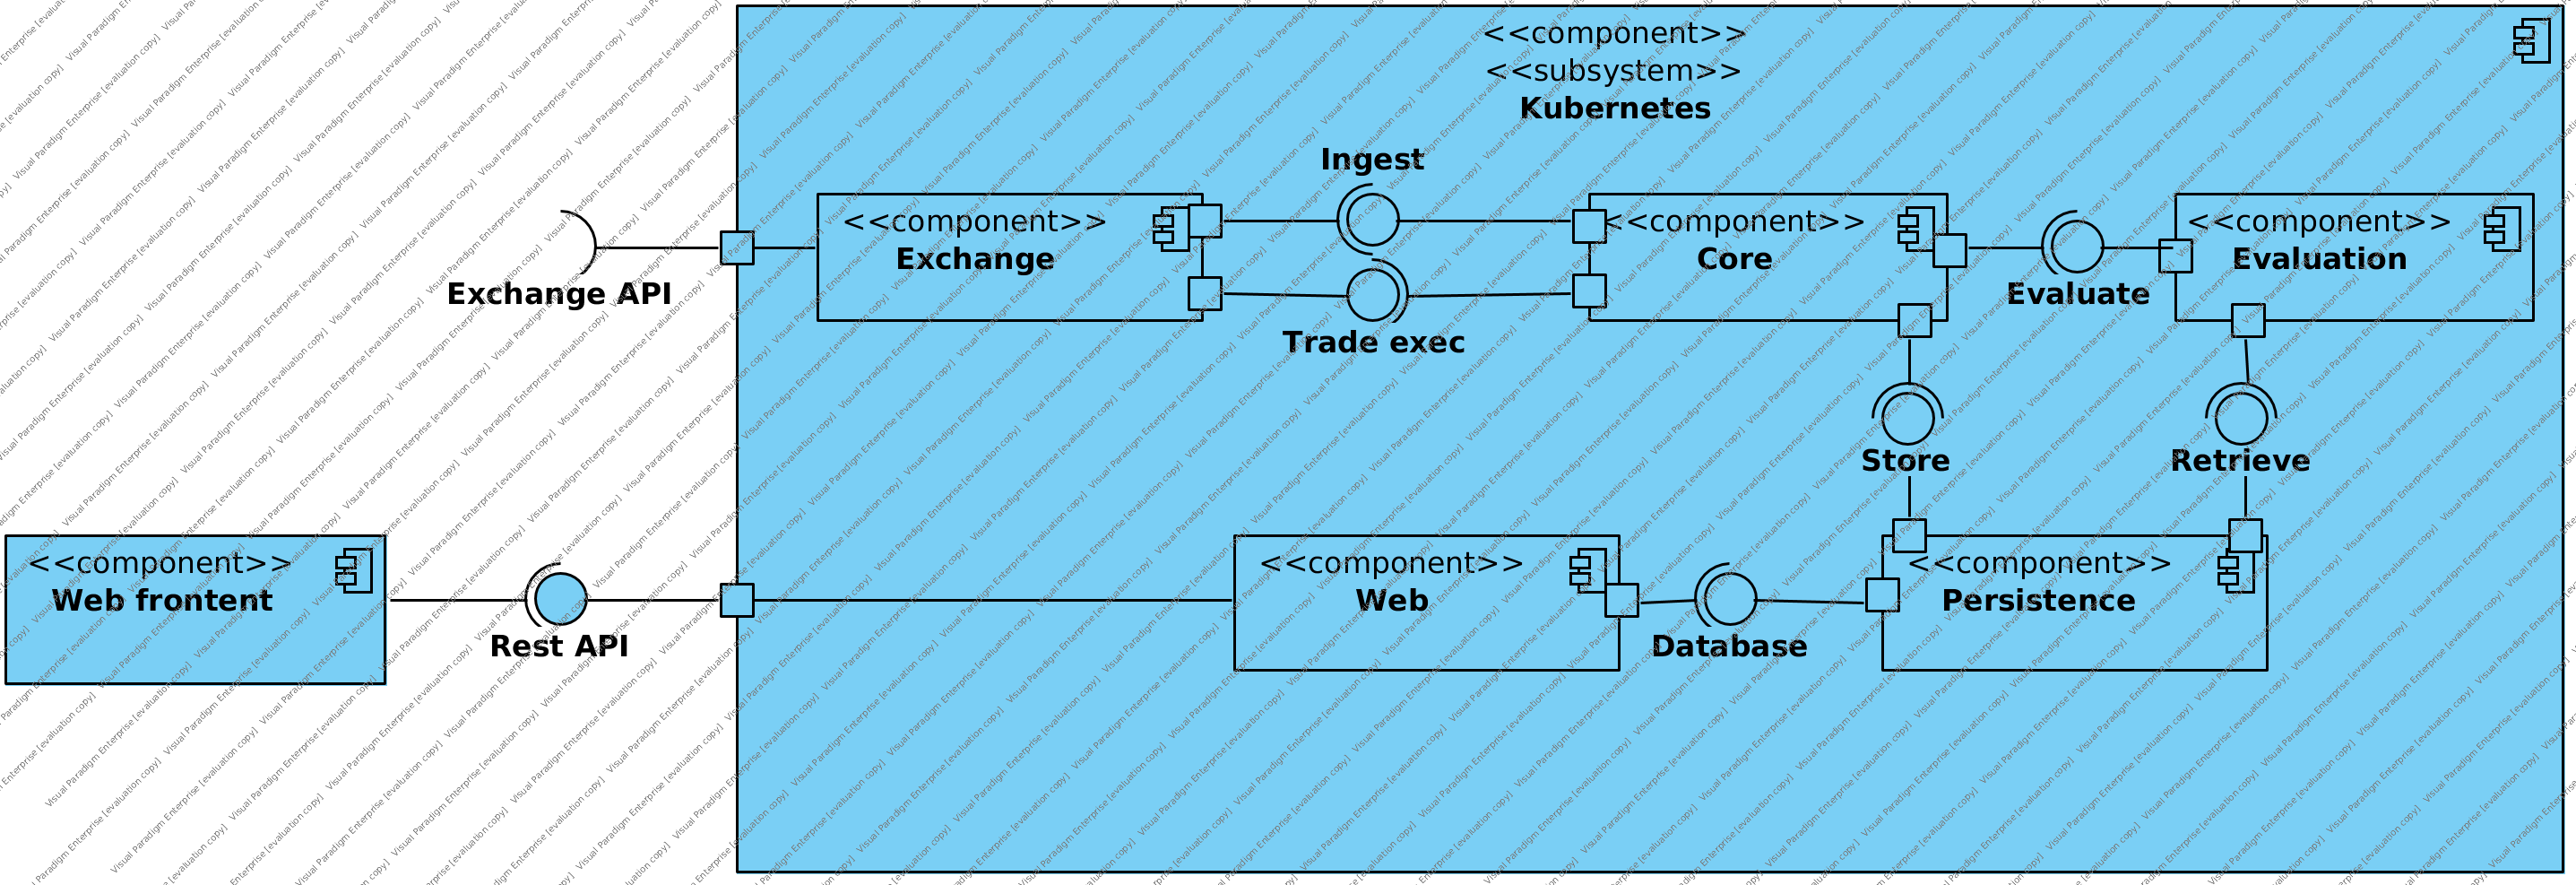
\includegraphics[width=\textwidth]{obrazky-figures/comp.png}
    \caption{Component diagram of basic architecture}
    \label{img:arch}
\end{figure}


\section{Component design}
By using Kubernetes we virtualized the computing environment. The environment as perceived by individual components
will just be a set of connected Docker containers with access to DNS server, that contains information about other components.
Kubernetes also provides virtualized network environment, making it appear as if all containers were on a same network.

This fact greatly simplifies architectural challenges. The only architectural challenge remaining, is the definition
of how will the application components be connected and communicate. While the actual communication protocol is
defined later in this chapter, here we are interested in more conceptual approach.

Application is divided into several components:
\begin{itemize}
    \item Web component - Provides a web interface for users' inetraction with the system, and interacts with the database
    \item Core component - Accepts input from users, incoming data from exchanges, decides when to evaluate strategies, and when to create orders on exchanges
    \item Evaluation component - Evaluates strategies based on requests from Core service
    \item Persistence component - Stores tick data and user data upon provided by core service, and provides this data to all services if necessary
    \item Exchange components - Each of these components serves as an adapter, that connects to external exchange API, and
    maps its specific API onto internal communication channels.
\end{itemize}

\begin{figure}[H]
    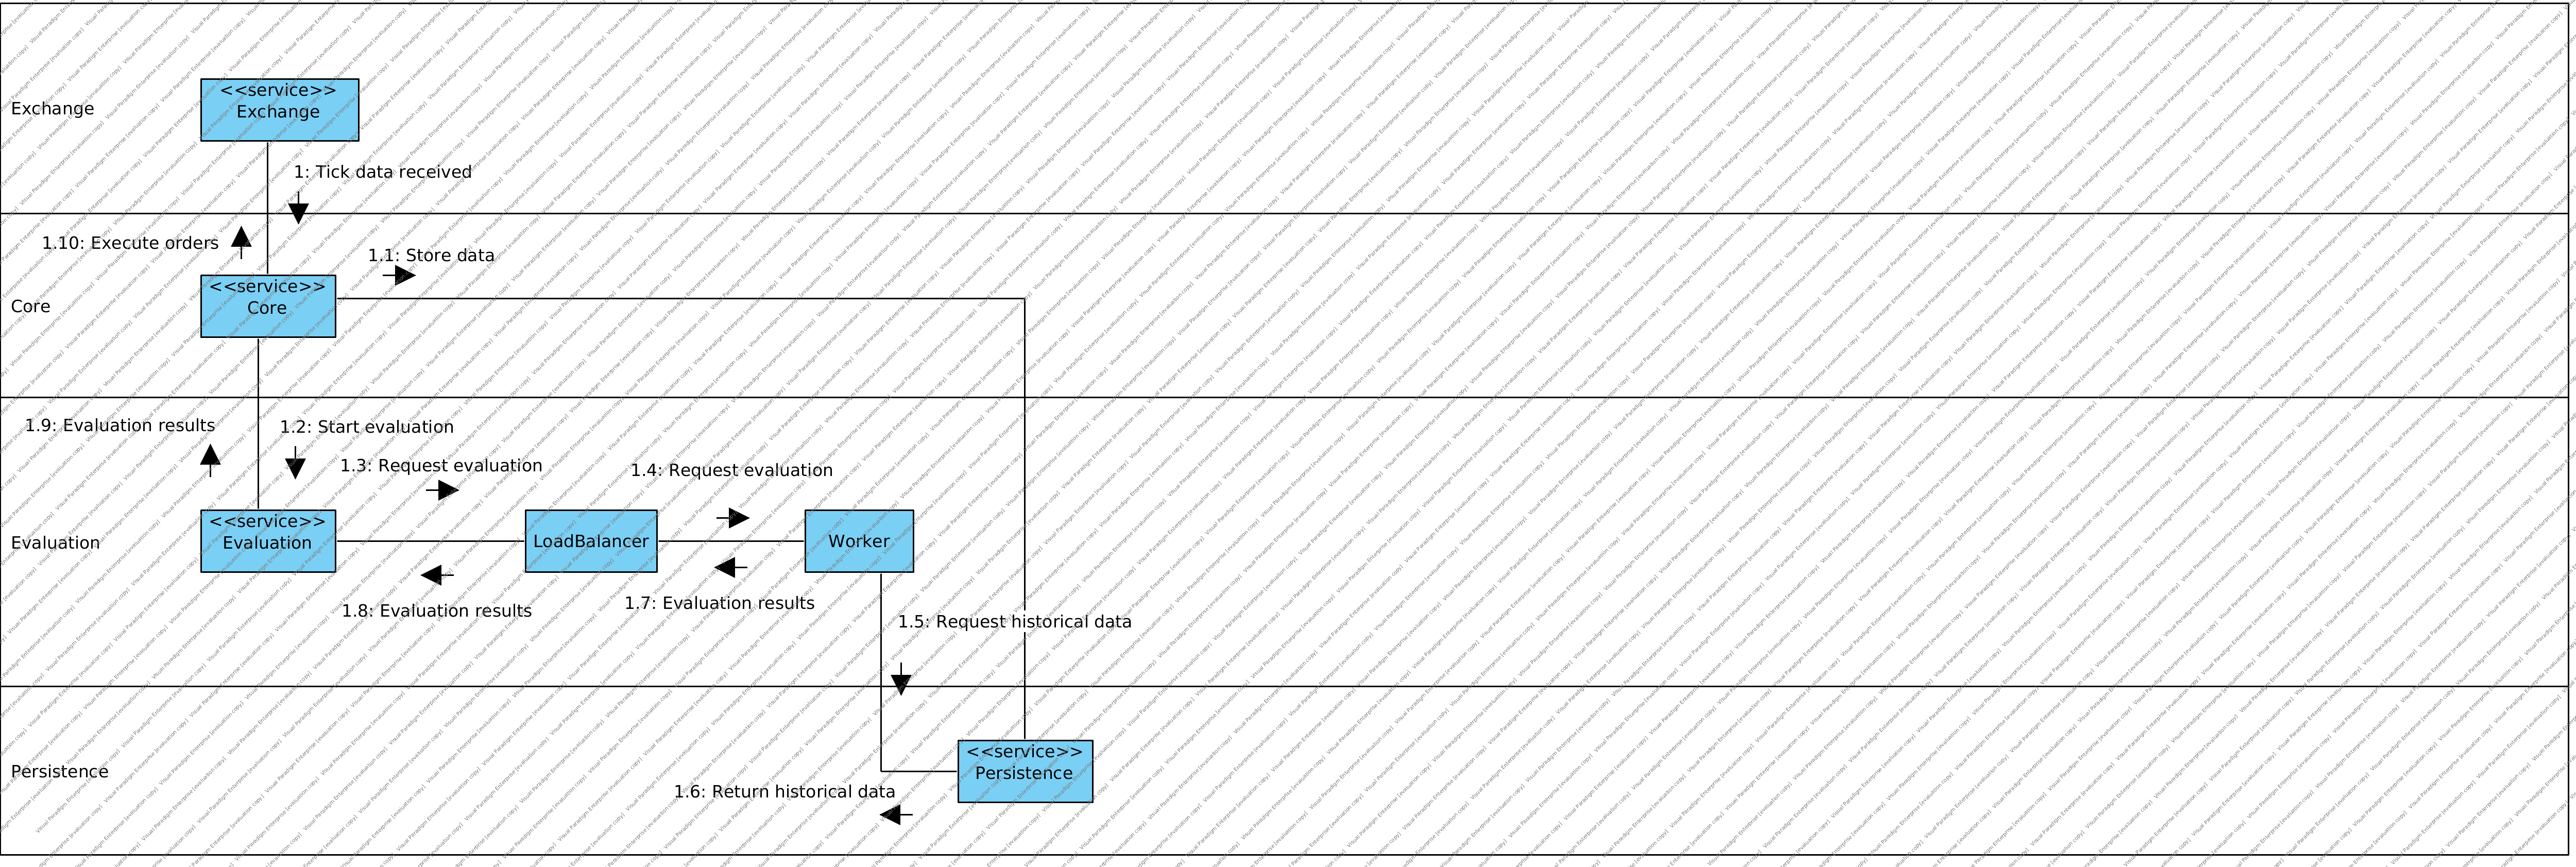
\includegraphics[width=\textwidth]{obrazky-figures/serv_comm.png}
    \caption{Service communication diagram}
    \label{img:service_comm}
\end{figure}

\autoref{img:service_comm} shows a communication diagram that describes communication between individual services, that
will occur in response to receiving new financial data from an exchange. The system will store this information
into persistent storage for later use, and if the information is up to date, it will initiate strategy evaluation
for strategies applied to currency of incoming data.

\subsection{Individual component architecture}
Each of these services will be comprised of one or more kubernetes \kubecomp{service}-\kubecomp{deployment} pairs. The
\kubecomp{service} part will ensure availability of information about individual pods on kubernetes' internal DNS server.
The \kubecomp{deployment} part will ensure the availability of actual pods.

Each service will be comprised of one ore more \kubecomp{pods} that will be managed by \kubecomp{deployment}. Each \kubecomp{pod}
will contain base communication actor from \verb|actix-comm| library, and several other actors to support communication with other services. In addition to
these supporting actors, it will also contain varying number of actors, that will collectively implement
the desired functionality of a particular component.

\section{Communication, actix-comm and actix-arch}
\label{section:actix_comm}
As described earlier the Actix library does not provide tools for communication between actors on different machines. One of the
goals of this thesis was to design \& implement a library that would facilitate this functionality. The resulting library
should be usable by other projects.

\subsection{Underlying protocol}
We chose to use ZeroMQ\cite{hintjens2011} as an underlying protocol instead of TCP/UDP because of several factors. The ZeroMQ can be used over
many different transport types, including TCP, UDP, Unix pipes, PGM or shared memory. Another benefit is the added flexibility; While
TCP requires establishing connection in a particular order (Bind then Connect), ZeroMQ does not have similar constraints.

Another possible approach would be usage of HTTP and/or Websockets. While these 2 communication protocols would probably
satisfy the requirements, ZeroMQ was specifically designed for low-latency, low-overhead applications and seemed
like a better fit into the global system architecture.

\subsubsection{ZeroMQ}
ZeroMQ is an asynchronous message-based communication library. It is aimed at low-latency distributed systems, and does not require a centralized
message broker. It provides primitives for implementing different communication patterns. Our library
will utilize 2 of these communication patterns.

The Router-Dealer socket types are used for asynchronous request-reply communication pattern, and our library uses
them to implement \actor{Request} and \actor{Reply} actors respectively, which collectively implement described communication pattern.
This type of communication is then used

The Pub-Sub socket types are used for publish-subscribe communication pattern. This communication pattern is implemented
by \actor{Publish} and \actor{Subscribe} actors.


\subsection{Library interface}
Because the library is intended to be used exclusively with the Actix framework, the only provided interface will be in form
of a several actors. These actors will respond to a set of messages that are also exported by the library.
The implementation of additional functionality by creating a set of actors \& messages is is very common within the Actix ecosystem.
For example, the actix-web library, which is used to implement the web application, is also built with similar approach

Upon Receiving \msg{SendRequest} message, the \actor{Request} actor sends actual message(which is stored inside the
\msg{SendRequest}) to a remote machine, along with an unique identifier. It then stores
this information along with notification token into its state, and returns other half of the notification token.
This token denotes future response to request that was just send over the network.


The \actor{Reply} actor responds to \textbf{Register} message, which is used for registering another actor
as a recipient of some message type. Then, whenever the \textbf{Reply} actor receives a message of said type, the message
is forwarded to registered actor.

The \actor{Publish} \actor{Subscribe} actors operate similarly to \actor{Request}, \actor{Reply} actors respectively,
but they do not send or receive message responses.

\subsection{Communication protocol}
Each of the defined communication actors contains one primary ZeroMQ socket that is used for receiving and sending messages
to other components. The actual communication protocols vary between individual actor types
\begin{figure}[H]
    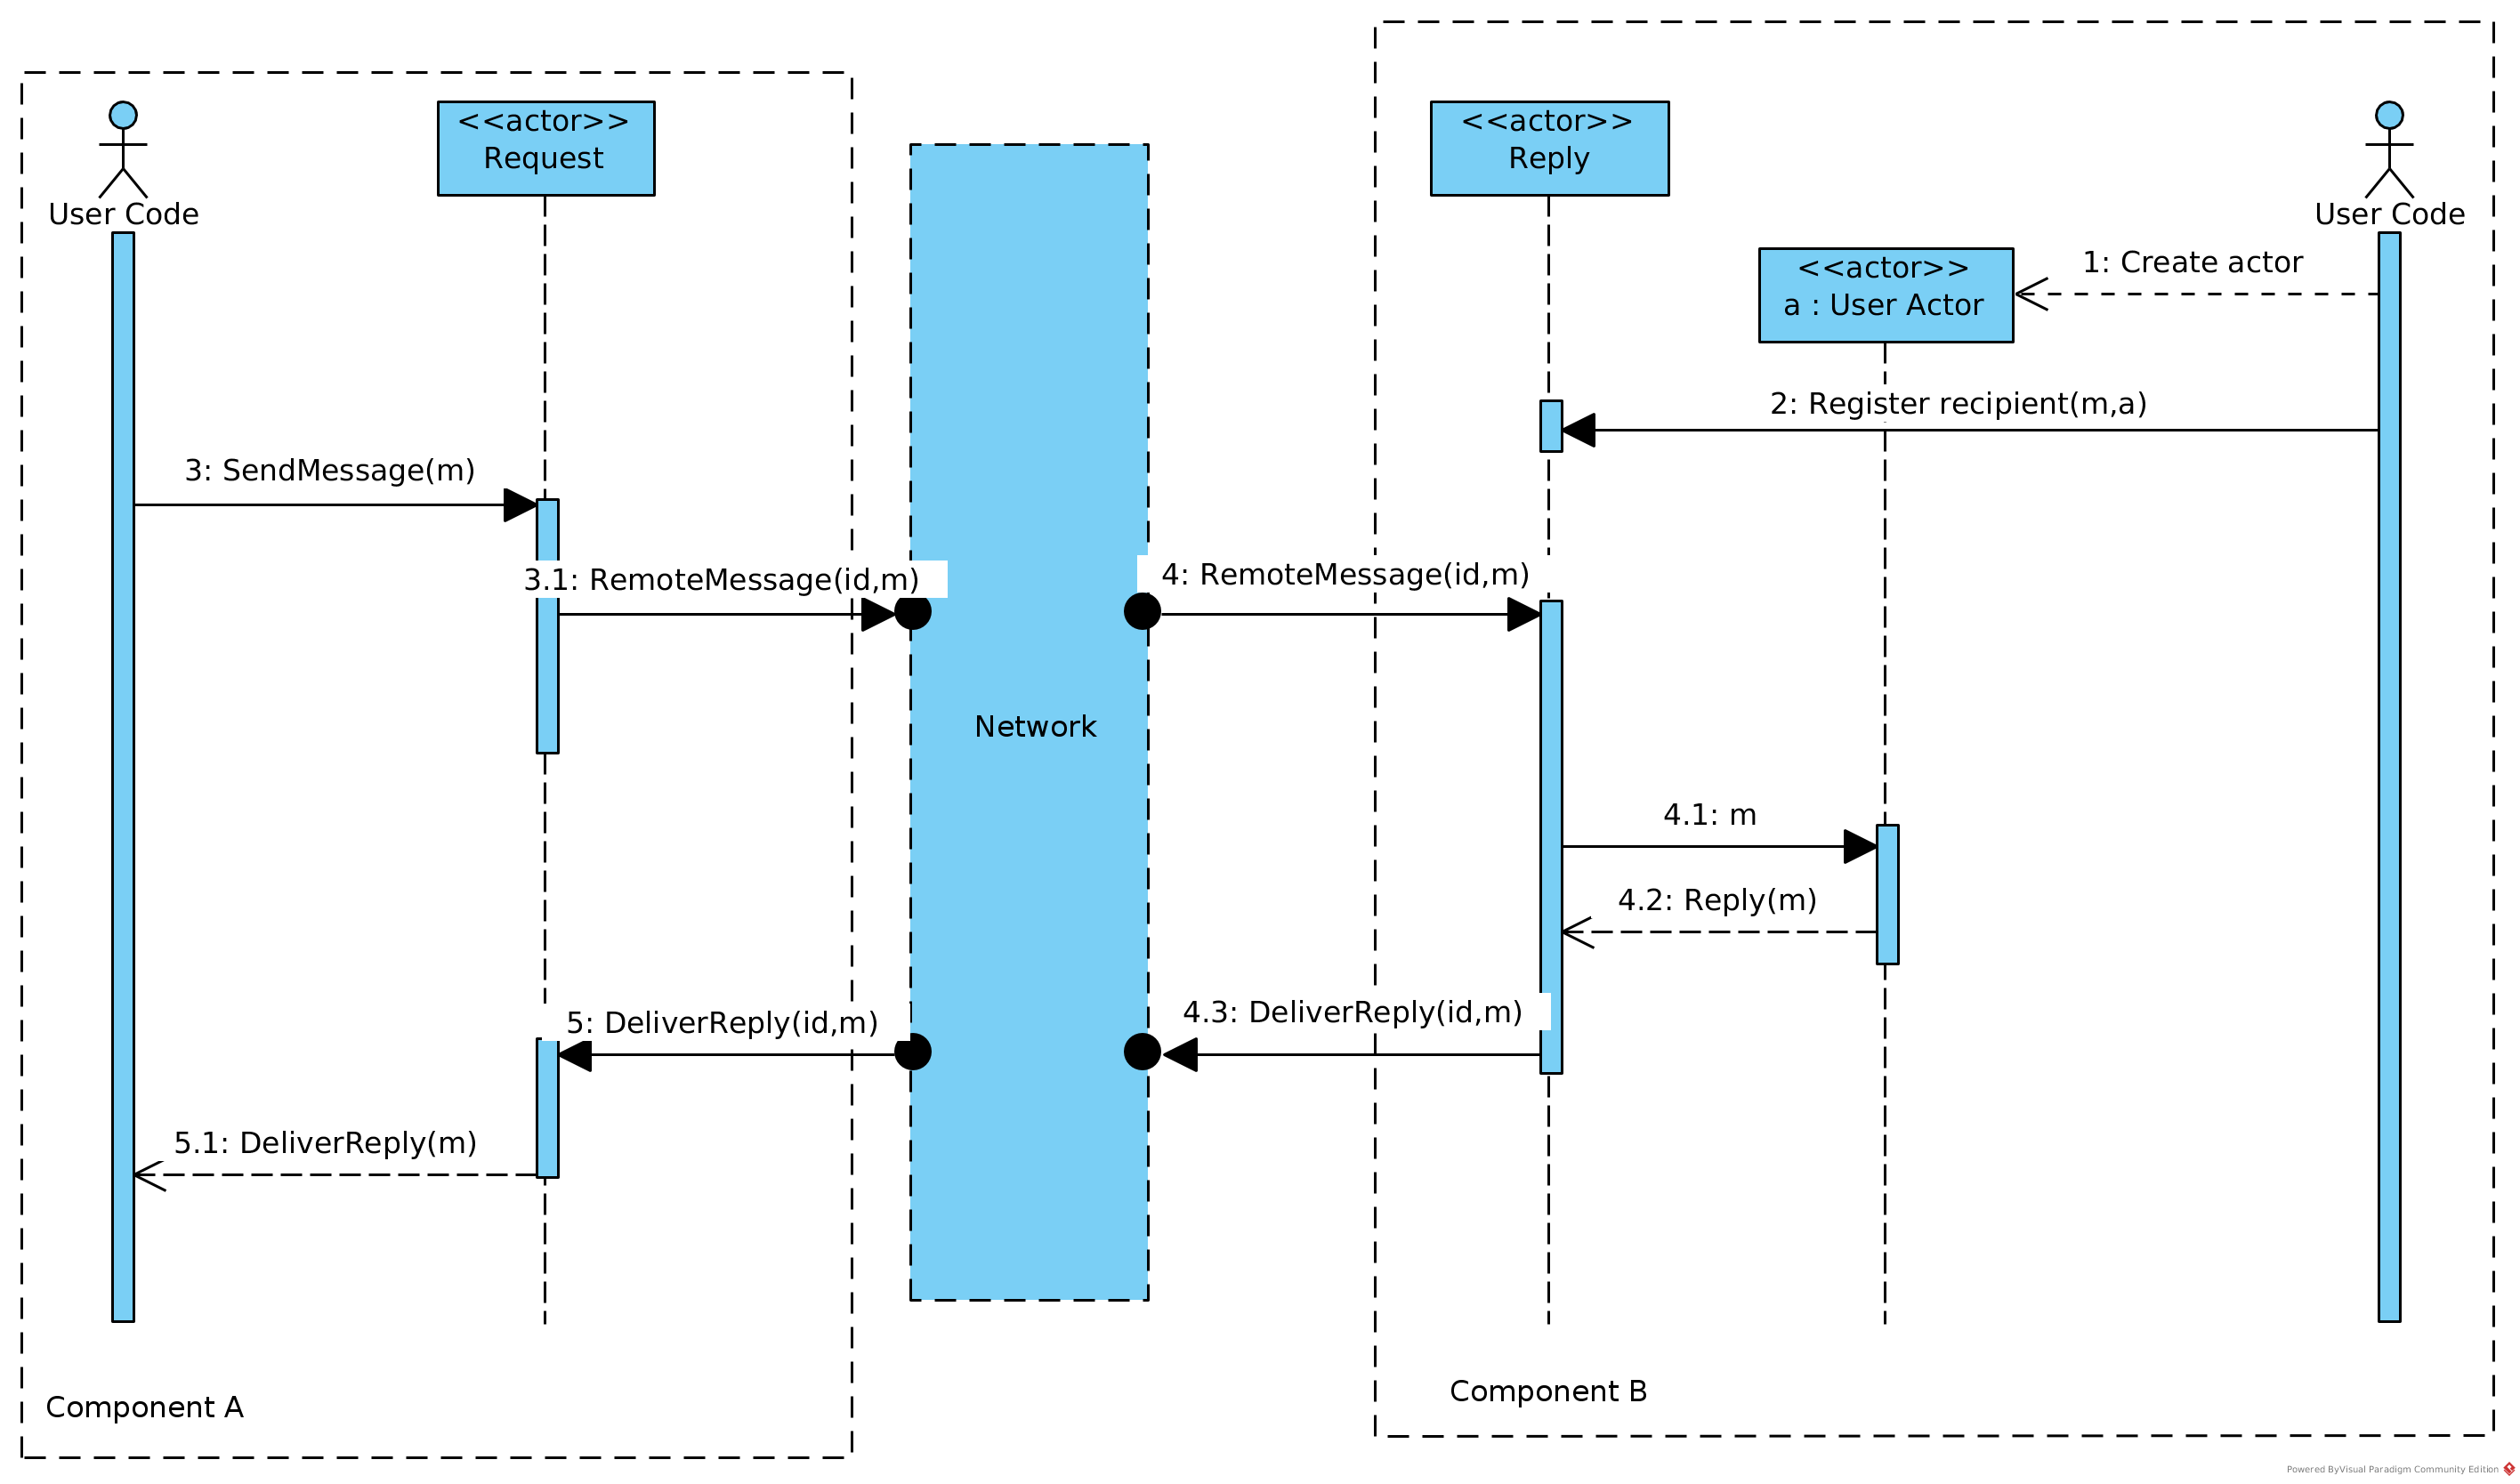
\includegraphics[width=\textwidth]{obrazky-figures/actix_net_comm.png}
    \caption{actix-comm communication}
    \label{img:actix_comm}
\end{figure}

In \autoref{img:actix_comm} you can see simple sequence diagram containing basic request-reply communication pattern.
The diagram contains 2 component. The component A contains a  \actor{Request} actor, that is used to send request to
component B, which contains \actor{Reply} actor and another, programmer defined, custom actor.
The user code in component B first
registers the user actor as a recipient of message type M. Then , the user code in component A sends a \msg{SendRequest}
to its \actor{Request} actor. It then stores some information about the message into its local state, and sends message
data along with its type to ZeroMQ socket.

After the \actor{Reply} actor in component B receives this message, it forwards the message to actor registered earlier,
and upon a response from this actor, it sends response along with metadata received earlier back to ZeroMQ socket.

Then, upon receiving the response, the \actor{Request} actor uses provided metadata to get appropriate notification
token from its local state, and uses it to notify originating code about the response.

\subsection{Message format, actor state}
Since we are using a language with extremely strong static type system, we decided to leverage this type syystem in much
of the library implementation. This reliance on static typing has made a whole class of errors impossible, but there
are some drawbacks to this approach. Since the data we send over the network is jsut a sequence of bytes, and our system
deals exclusively in strongly typed messages, we must solve the problem of serializing and deserializing messages into bytes.

\subsubsection{Serialization}
The serialization was very simple to solve. We utilized the \verb|serde| library, which is main data serialization and deserialization
library in rust, and supports many data formats. For the development purposes, we utilize JSON as a serialized data format,
but for production use, we aim to replace it with MsgPack in order to reduce serialization overhead.

\subsubsection{Deserialization}
The main problem of deserialization was determining what datatype should a message be deserialized into.
We solved this by including unique type identifier with each message sent over the network, This identifier relies
on information provided by standard library intrinsic function, which utilizes data provided by compiler.
Using this information, and a clever trick utilizing type erasure we were able to safely bridge typed and untyped
parts of this library.

\subsubsection{Actor state}
Each actor in this library stores notification tokens representing running tasks inside its state. Each request also
has a unique numeric identifier associated with it. This identifier is sent over the network, and expected to be
send along with the response. After receiving the identifier, the local actor finds notification token associated
with it, and uses it to notify user code about request completion.

These notification tokens are implemented in form of single-shot channels provided by the \verb|futures| library.

\subsection{Actix-arch}
Is a library that was built on top of \verb|actix-comm| simplify development of individual components. It contains implementations
from common communication patterns, and components to support the development of communicating applications.

\subsubsection{Service abstraction}
Since most common communication pattern is Request-Response, this component was created to support this type of communication.
It consists of 3 parts. The \trait{ServiceInfo} trait, that is used for declaring crucial information about the service, like
hostname, on which the service is available, and types of request and response.

%@formatter:off
\begin{code}[language=rust,label={svcinfo_trait},caption={ServiceInfo trait definition}]
pub trait ServiceInfo: 'static + Debug {
    type RequestType: Remotable + Debug;
    type ResponseType: Remotable + Debug;
    const ENDPOINT: &'static str;
}
\end{code}
%@formatter:on

Two other components are the \type{ServiceHandler} and \type{ServiceConnection} structs, which are generic over type paramenter
S, that must implement \trait{ServiceInfo} trait. The \type{ServiceHandler} struct has a register method, which can be used to register a handler of service messages.
Both of these structs internally use ZeroMQ actors defined in \verb|actix-comm| library, namely the \actor{Request} and \actor{Reply} actors.

\subsubsection{Publish - subscribe abstraction}
Is an abstraction for implementing Publish-Subscribe data flows.
Is analogous to Service abstraction, utilizing 3 parts. The \trait{EndpointInfo} trait defines the hostname, on which
the binding endpoint can be found, its associated type \type{FanType} can be either \type{FanOut} or \type{FanIn},
and defines, which part of the communication channels binds to an address, and which connects to it.
With \type{FanIn}, the subscriber binds to a port, and multiple publishers connect to it (used for receiving data from multiple exchange adapters),
and with \type{FanOut}, the publisher binds to a socket, and subscribers connect to it.

%@formatter:off
\begin{code}[language=rust,label={endpointinfo_trait},caption={EndpointInfo trait definition}]
pub trait EndpointInfo {
    type MsgType: RemoteMessage<Result=()> + Remotable;
    type FanType: FanType = FanOut;
    const ENDPOINT: &'static str;
}
\end{code}
%@formatter:on

The \type{Publisher} and \type{Subscriber} actors are generic over type parameter E, that must implement the \trait{EndpointInfo}
trait, and contain methods for publishing and subscribing to updates respectively.

\subsubsection{Service load balancing}
Other component necessary for our designed system was a way to perform load balancing for Service handlers.
This will be mainly used in the strategy evaluation component, since this component will probably result in most
of the computing load.

This component is implemented as 2 actors: the \actor{LoadBalancer} and \actor{WorkerProxy}, which both have one type
parameter S that must implement ServiceInfo. The \actor{LoadBalancer} binds 2 ServiceHandlers to single port.
The first one is used for receiving service requests from client, and the second one is used for receiving messages from workers.

The \actor{WorkerProxy} internally contains a \type{ServiceConnection}, that connects to \actor{LoadBalancer}, and periodically subscribes
for work. If \actor{LoadBalancer} does not have any work available, it sends an empty response to \actor{WorkerProxy},
or, if available, it sends a work unit to this worker. The \actor{WorkerProxy} then sends received work to internal
worker implementation, and after finishing, sends result to \actor{LoadBalancer} as a separate request, that is also used
for requesting more work units.

Therefore, the \actor{LoadBalancer} therefore serves as a load balancing broker, which performs rendezvous between
available workers and work units.
\section{Data storage}
Another crucial aspect of designed system is the storage of both the financial data and general system data.
These 2 types of data have different storage requirements.


\subsection{System data}
We use this term to describe data that denotes the system state. This means User accounts, and data associated with
these accounts. This set of data can bea easily mapped onto the relational model, and therefore we chose to store it
in relational database.

There are several very popular relational databases, each with their own advantages and disadvantages. We elected to
use PostgreSQL\footnote{https://www.postgresql.org/} because of its vibrant open source community, custom extensions, and support of large
part of modern SQL standards \cite{sql_comp}.

The system data is described by following ER diagram:
\begin{figure}[H]
    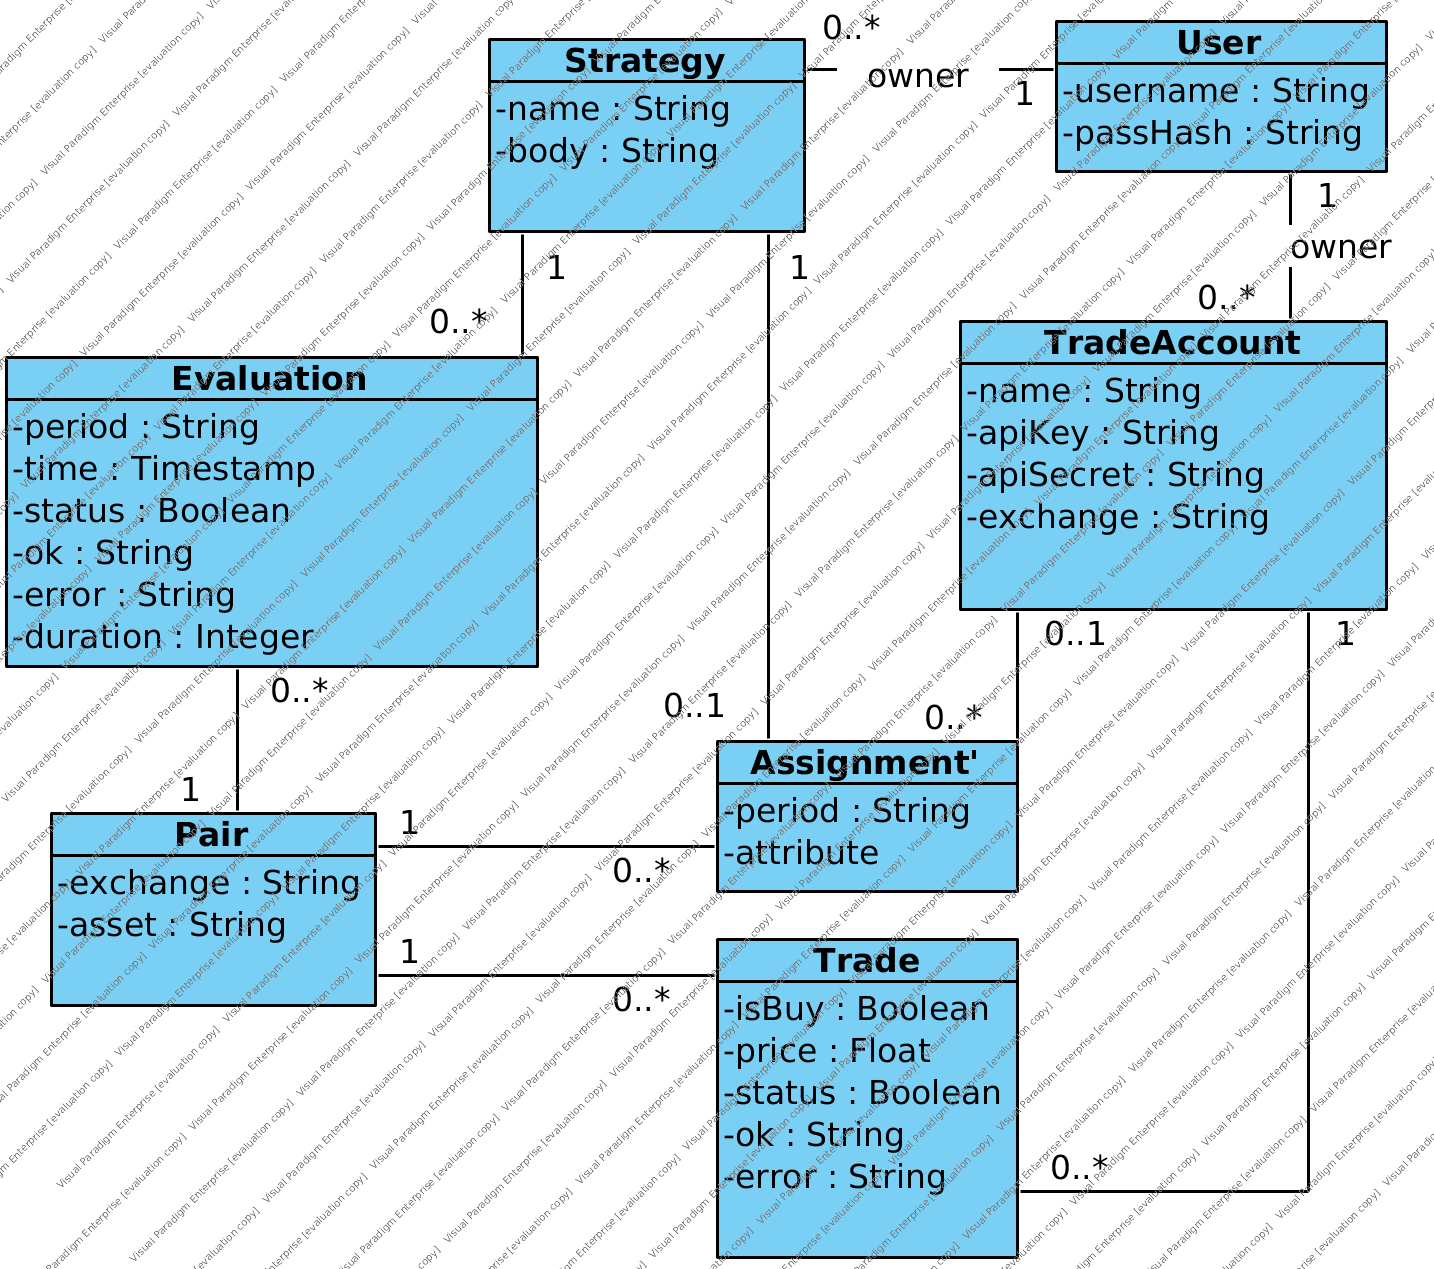
\includegraphics[width=\textwidth]{obrazky-figures/ERD.png}
    \caption{Entity-Relationship diagram of system data}
    \label{img:arch}
\end{figure}

\subsection{Asset data}
\label{section:ohlc}
Along with the system data, we also need to store information about individual assets that we receive from exchanges.
This data has a particular format. It consists of periodic updates about an asset, with each update containing several
prices and some additional information.

These prices are:
\begin{itemize}
    \item{Open - } Price, that was used in first transaction in this time interval
    \item{High - } Highest price that was used in transaction in this time interval
    \item{Low - }  Lowest price that was used in transaction in this interval
    \item{Close -} Price, that was used in last transaction in this time interval
\end{itemize}

In adition the these price, each interval is associated with its starting timestamp, and cumulative volume
of executed trades. We will refer to this type of data as OHLC data, based on the OHLC chart which is used for displaying
these datasets \footnote{https://www.investopedia.com/terms/o/ohlcchart.asp}.

There are several requirements put on storage solution that will be used for storing the OHLC data. Since this data is received periodically,
every minute, and is received for each asset, the chosen storage solution will have to support large insert rates. For example,
even if we support only the Bitfinex\footnote{https://www.bitfinex.com/} exchange, we will have to store OHLC data for more than 200 assets,
most of which are updated every 20 seconds. This puts a requirement of 10 inserted rows per second onto our storage solution.

Another aspect is retrieval of the data. We need to be able to retrieve several hundred rows from last inserted data with
low latency, and retrieve older data without hard latency requirements. Also, we need to perform periodical maintenance
of the data set for the purpose of effective strategy execution (eg. filling missing data points). This task would be
much easier, if we had full SQL support.


\subsection{Evaluated storage architectures}
As mentioned earlier, we chose to utilize PostgreSQL to store system data. This decision was mainly influenced by the
ability to use modern SQL, and the ability to extend the database with custom, and commercial extensions.

As for the storage of asset data, if we have to satisfy constraints outlined earlier, we have several choices. These
choices will have to support large insert rates, fast retrieval of latest data, and preserve these properties even
when amount of stored data grow to the point when it can no longer be stored in memory. These requirements are common
among applications that deal with a steady stream of time dependant data ( also called time-series data).

The conceptual architectures that satisfy these requirements are:
\begin{itemize}
    \item{Cloud database} - Utilizes a database provided by external provider, that is optimized
    for large workloads.
    \item{Distributed database} - This approach utilizes a distributed - multi-master database,
    that allows us to utilize several machines for storing and retrieving data

    \item{Relational database with shared tables} - This approach utilizes relational database, in which
    we store the data in several sub-tables of limited size. Insert rates are improved, because indexes
    are smaller.
\end{itemize}

\subsection{Evaluated solutions}
We evaluated several technologies, each based on an architecture outlined earlier.
\subsubsection{Cloud database}
As for external databases provided by cloud providers, we evaluated Google's and Amazon's offering.
Google provides their Cloud Bigtable database, that potentially could be used for our purposes. It provides
apache HBase API, and is basically a key-value store. But, even if it provides very impressive perofrmance,
the pricing of this technology is very steep, and thus we elected to not use this technology for now.

Last year amazon announced their Timestream database, that seems it could possibly support our usecase, but this
technology is till in beta, and not available to public. In the future, we might revisit this technology.

\subsubsection{Distributed database}
We evaluated Cassandra, and ScyllaDB distributed databases. Both of these technologies
provide same API, each of them provides impressive performance, and ability to scale to multiple nodes.
However, ScyllaDB has lower memory requirements and lower latencies, thus it was preferred.

Both of these databases support only subset of SQL, which we found lacking. However, the
performance achieved vas very impressive, and if, in the future, we need to achieve better performance,
the migration to ScyllaDB would be a great way to achieve it.
\subsubsection{Relational database}
Since we are using PostgreSQL for storing system data, we could also store the asset data in this database.
This would greatly simplify the system. However, in order to achieve performance figures required, we need to
utilize table partitioning. We evaluated TimescaleDB extension, that implements table partitioning,
and provides extensive suite of supporting functions for working with time-series data.

\subsubsection{Chosen technologies}
The ease of use, and relatively satisfying performance made the PostgreSQL + TimescaleDB combination the
chosen technology for storing the asset data. If this solution does not provide adequate peroformance
in the future, we will probably migrate to using ScyllaDB, along with separate component for data maintenance,
that is currently performed by utilizing andvanced SQL queries with PostgreSQL.


\section{Web}
As mentioned earlier, we elected to implement the web application with the single-page approach. This requires dividing
the application into 2 parts. The Backend part will run on the server, and provide information to the Frontend running on the
clients web browser.

\subsection{Backend}
The backend part of the web application is implemented in \verb|actix-web| library, which, like many other parts of this project,
is built upon \verb|actix| and its implementation of the actor model. This component will provide several REST endpoints
for working with system resources like strategies, trader accounts, or strategy assignments. Internally,
these endpoints should perform validation of input data, and execute database queries, which modify the state of the system.

Other languages were not considered for this task, because utilizing them would mean that definitions of stored entities
would have to be duplicated, and the cost of duplication would not be outweighed by the benefits provided, since
the Backend part of the application is relatively small.

\subsection{Frontend}
For implementation of the Frontend part of the application, we evaluated several popular technologies.

\subsubsection{Polymer}
Is a library developed by Google. It utilizes custom webcomponents\footnote{https://www.webcomponents.org/}, Shadow DOM and HTML Templating technologies
to achieve remarkable set of functionality with only a small extension build upon common web standards, that all major
browsers implement. This technology is based on the \verb|lit-html| library, which can be used for creating HTML templates directly from
javascript. However, using polymer requires custom command line tool, in order to build applications made with this technology.

\subsubsection{Angular}
One of the most popular web frameworks, provides large amount of functionality. It does not use webcomponents or shadow dom,
due to the fact that these advances came after it was created, since its predecessor was first of these kinds of libraries.
It provides two-way databinding, utilizes MVC architecture and should be considered to be a framework instead of a library
due to opinionated nature of this library. It uses Typescript instead of Javascript as main application implementation language.

\subsubsection{React}
Is is component based user interface library, with one of its targets being the web browser DOM. Other targets
include Android , iOS, UWP , and are implemented in React-native branch of this library. React uses
JSX indstead of plain javascript. This language is an extension to javascript, that allows programmer to write inline
HTML inside normal javascript code, improving readability. React does not attempt to provide general application framework,
its only targeted at building user interfaces.It is based on its virtual-DOM architecture. In this approach
the entire application is rendered into memory representation of the resulting DOM, that is then compared to actual rendered
DOM tree, and only changes are applied. This reduces number of updates that must be performed, increasing rendering performance
at the cost of memory usage.

\subsubsection{Flux \& Redux}
One of most important concepts used in React is the uni-directional data flow. Data flows
from components to their children, and notifications from children to parents.
To support this paradigm, we utilize the Flux architecture. In this architecture there are \textit{actions}, that flow through the
central \textit{dispatcher} to a \textit{store}, and changes in the store are propagated back to view. In react,
this propagation is performed through component properties. This approach is similar to observer pattern\footnote{https://en.wikipedia.org/wiki/Observer\_pattern}
With this architecture, the properties passed to a components are immutable. Only way the application state can be affected is
through sending \textit{actions} to dispatcher.

Redux is the most well known implementation of this pattern. It features a single store, and dispatchers are
called reducers. The reducers are pure functions, that respond to actions, and based on them modify this single source of truth.


\subsection{Frontend application}
After experimenting with each of these technologies, the \textbf{React} library with \textbf{Redux} was chosen ast the most suited technology for creating the \textit{frontend}
part of the web application.
Another aspect of the \textit{frontend} part of the application to consider is the user experience. The user
must be able to:
\begin{itemize}
    \item Create an account
    \item Login \& Log out
    \item Create \& edit strategies and exchange trading accounts
    \item Assign strategies and trading accounts to assets
    \item Visualize the results of strategy evaluation and executed trades
\end{itemize}

\section{Exchange adapters}
While all cryptocurrency exchanges use similar technologies to implement their APIs, each of them is different. To reduce
complexity of the system, these differences must be resolved at the edge of our system, and should not permeate into other
components. To bridge the gap between external APIs, and internal communication, the system contains adapter component
for each exchange.

This component connects to real-time websocket API in order to receive notifications about market updates,
then translates this data into OHLC format, and sends it to the \kubecomp{core} component.
It also exposes a service endpoint for querying account state (wallet balances), and executing trades, to which the
\kubecomp{core}'s trader actor connects.

\section{Strategies}
\label{design:eval}
In \autoref{chapter:current_state} we have described several implementations of automatic trading systems. Each one of them
utilized some kind of programming language to define a trading strategy. In this regard, our system is very similar to others.

The system will have to support execution of user-written code. This fact poses a security concern. Because the user
written code can perform arbitrary actions permitted by given programming language, we must carefully choose the programming
language that will be used. Because implemented strategy will be operating with large amount of financial data, another
concern is performance. And finally, since the intended users of this application are not programmers, the chosen language
should be easy to use for beginners.

\subsection{Language choice}
These requirements severely limit possible choices. We can't accept user-compiled code, because of security concerns.
Compiled languages like C/C++ are not acceptable because of large amount of infrastructure needed to support
on-demand compilation of user written strategies.

Managed languages like Java or C\# are a better choice, but they still require large runtimes with long start up times, therefore
are not well suited for running short-lived scripts.

Scripting languages like Lua, Python or JavaScript seem like the best choice for this goal, with the drawback of
reduced performance.

\subsection{Lua}
Ultimately, the Lua language was chosen as a primary language for implementing user defined strategies. There were several
key properties, which caused this decision.

\begin{itemize}
    \item Embeddability - Lua runtime is smaller than 256Kb, has virtually no start up time and can be embedded in application.
    as a simple library. In comparison, neither Python nor JavaScript runtimes can be embedded in the application, and both
    require large standard libraries
    \item Extendability - Basic lua standard library can be easily extended with code written in host language.
    \item Expressive power - While extremely simple, lua provides tools to model virtually any programming paradigm with ease
    \item Speed - While lua is a scripting language, that can't possibly compete with compiled language in this space,
    it is one of the fastest scripting languages available.
\end{itemize}

\subsection{Safety}
By using an intepreted language for implementation of user strategies, we have successfully eliminated a whole
class of risks. By using a safe language, the probability of user code crashing the executing process is virtually
none. However, there still are several safety issues, that have to be resolved, even with using an interpreted language.

\subsubsection{Sandbox}
As a basic strategy for ensuring the safety of strategy execution, we chose to utilize a sandboxing mechanism.
This mechanism is supported by LUA very well. The sandbox mechanism consists of replacing the global environment table
with a table, that contains only functions deemed safe when executing user code. This simple replacement
restricts access to unsafe functions like \verb|read|, removing the ability to of an malicious to to
affect our system

\subsubsection{Execution control}
Another attack vector considered was the ability of an attacker to perform A Denial-of-Service(DOS) attack by
submitting a strategy, that never terminates. Upon the start of evalauation, this strategy would lock
currently evaluation actor, reducing the amount of available actors for strategy evaluation. After
sufficient amount of attempts, this would leave no available actors, and then, the system would be unable
to function.


To ensure this attack is not possible, we limit number of LUA instructions that a particular strategy can execute.
This is done by utilizing the \verb|debug.sethook| function.

\subsection{Access to information}
Method for strategy evaluation described so far should provide safe, and performant
way for users to write custom code, that can be run inside our system. However, we must allow this code to access the
financial data, and provide some kind of library for supporting the strategies.

We expose a vector of OHLC data items inside the \verb|__ohlc| global variable. Each item in this vector
has methods to access individual prices described in the \autoref{section:ohlc}.

We also expose a set of functions implementing indicators for Technical analysis\footnote{https://en.wikipedia.org/wiki/Technical\_analysis}.
These are available inside the \verb|ta| global table.


\subsection{Technical analysis library}
This library is contained in a global variable named \verb|ta|. It contains most common technical indicators used in
trading. These indicators are mathematical functions applied upon a sequence of OHLC data, mostly
denoting some statistical property of the data. Implemented indicators are:
\begin{itemize}
    \item \verb|sma| - Simple moving average
    \item \verb|ema| - Exponential moving average
    \item \verb|macd| - Moving average convergence-divergence
    \item \verb|rsi| - Relative strength index
    \item \verb|tr| - True range
    \item \verb|atr| - Average true range
    \item \verb|min| - Minimum value
    \item \verb|max| -  Maximum value
    \item \verb|fs| - Fast stochastic oscillator
    \item \verb|ss| - Slow stochastic oscillator
\end{itemize}
Each of these indicator has a precise mathematical definition, and aims to model an aspect of the market, but explaining
these details is outside the scope of this thesis.

These indicators can be accessed by calling a function in the \verb|ta| global table with appropriate number of arguments.
Returned object provides a call operator, that can be used for receiving the indicator value.



\section{Evaluation}
Since users can crate multiple strategies, and then apply these strategies to multiple different assets on different exchanges,
the amount of work associated with a single user can vary extremely. In addition to that, the number of users of our system can vary.
This variability of computational load on the system was primary reason for designing the system as a distributed application.

The service that is most affected by this variability is the strategy evaluation service. This service needs to
dynamically change the amount of used resources.


To implement this component, we will utilize the \actor{LoadBalancer} actor defined earlier.
This will require specific architecture. The service will be divided into 2 parts. The control and the worker layers.
The control layer will be a single Kubernetes pod, that will serve as an endpoint to rest of the system. It will receive
strategy evaluation requests from Core service, and will pass them to individual workers int the worker layer.
Each worker will be a single pod with multiple worker actors, each of which will register itself with control layer.

The control layer will also perform load balancing, ensuring that no single worker is over or underutilized.

\chapter{Implementation}

In this chapter, we aim to present current state of the implementation, outline the problems faced when trying to satisfy the
requirements outlined in previous chapters, what methodologies and approaches were taken to solve them, and also
point out some interesting aspects of the implementation. Another goal of this chapter is to present the "operations"
side of this project, meaning the processes used for building and deploying the system, since that was another
important part of the implementation

\section{Project structure}
Like any other larger project, this project is also structured into several subdirectories. The main subdirectory is \verb|code|,
which contains the code for system components, the \verb|common| library and several other
libraries in the \verb|deps| directory. The \verb|common| library groups dependencies that
are shared by all components, and re-exports them for easier access and centralized version selection. The \verb|deps| subdirectory contains
for \verb|actix-arch|, \verb|actix-comm|, \verb|db| libraries and other dependencies.

Then, the second core directory is the \verb|ops| directory, that contains scripts and configuration files
needed for deploying and managing the system.

The main directory contains \verb|Cargo.toml| file, that is used by the \textbf{cargo} tool. This root file
defines a workspace, and some configuration profiles for rust compilation. Each directory containing sub-project of
a library or an executable also contains the \verb|Cargo.toml| file.

The \verb|target| directory contains build artifacts created byu cargo, and is also used to store intermediate files produced by our custom build scripts, that
will be described in the following section.

\section{Building and deploying}
Thanks to the distributed architecture, the building and deployment processes also had to be modified with this choice in mind.

The rust language utilizes custom tool named \textbf{cargo} for building rust projects, and managing their dependencies.
Having single tool manage both build process and dependency management is extremely useful, but its not without drawbacks.
\textbf{Cargo} cannot be used for building anything else than rust projects, and while it allows to customization
of the build process by running pre-build custom scripts, it does not support customizing the build process with
any kind of post-build steps.

Therefore, to solve these drawbacks, we have to wrap cargo in a meta-build system, that would manage building
individual rust projects using \textbf{cargo}, and perform any  additional neccessary steps.

\subsection{Makefile meta-build management}
This meta-build system, does not have to do anything particularly complex, it only needs to track what projects
were changed, and depending on that information re-build, and re-deploy them.

These requirements are perfectly satisfied by the ancient \textbf{make} unix tool.
The project root contains the root Makefile, which references supporting makefiles stored in the \verb|ops/make/| directory.
It contains the \verb|deploy| target, that builds all custom components, creates new docker images from them,
re-evaluates the kubernetes configuration templates, and finally applies this configuration to currently active kubernetes cluster.


\subsubsection{Building a component}
One build target roughly corresponds to a \textbf{cargo} project, that produces an executable, and a docker container
that contains this executable. Implementation of this build process is in \verb|ops/make/App.mk| makefile. This makefile
invokes cargo in an appropriate subdirectory, it then creates a docker container image according to \verb|ops/docker/app.Dockerfile|,
and emits container name and container tag into a file in \verb|target/docker/| directory. This information is provided in a format
that will later be loaded into an environment variable, and used for substitution when building kubernetes
configuration templates.

\subsection{Kubernetes configuration templating}
This is very well known drawback of kubernetes. It does not support any kind of templating out of the box.
There are existing solutions, that solve this issue, but many of them do so with opinionated approach that is coupled
with some kind of package management.

We elected to perform this templating manually, inside the makefiles implementing the build process. For this purpose,
build of each component emits built docker image tag in the format of \verb|{COMPONENT}_IMAGE={IMAGE TAG}|.
Then, for each file in the \verb|ops/k8s| directory
the main makefile loads it, performs environment variable substitution using the \verb|envsubst| tool, and saves modified
file to \verb|target/k8s| directory. There are dependencies between these steps, which are also listed in the makefile, and
therefore it does not re-build components that were not modified.

Each image of a component is tagged with a special unique information identifying application version. Currently,
this is the first 10 characters of the sha256 hash of the binary, but in the future, this should be changed to current
git commit hash.

\subsection{Build targets}
Currently, the application is divided into 2 build targets. The \verb|web| build target contains the implementation
of the web application(both frontend and backend), and the \verb|app| build target contains the implementation
of every other component that in the system. This grouping is an artifact of how the system was developed, and in the
future should be resolved by moving each system component into separate build target.

\section{Component implementation}
Most of the application is written in pure rust, with the exception of the frontend part of the web application, which
is written in javascript. The project uses multiple advanced features of rust, that have not yet been stabilized, and
therefore requires a nightly toolchain. Currently, the project uses nightly toolchain from 2019-05-01. Main
reason for using a nightly toolchain with a specific version is the fact, that the implementation utilizes
async-await style programming, which has not yet been stabilized, recently had untergone
several changes. These features should be stabilized in several months.

The usage of asynchronous code is prevalent throughout the codebase. Almost every actix actor is written in a way, that requires
it to send and wait for message response when responding to a message itself. With synchronous code, this would mean, that
the throughput of the system would be very low. With asynchronous code, the actor will perform some synchronous actions,
will send messages other actors, and will then asynchronously wait for these messages. During this waiting, the actor
can respond to other messages, greatly improving throughput.

\subsection{Core component}
Core component is comprised of 3 main actors. As its name suggests, it implements the core system logic, and
other systems connect to it.

\subsubsection{Ingest}
The \actor{Ingest} actor binds a \actor{Subscriber} to a known port, and waits for publishers to connect to it.
The publishers are created by exchange adapters, and the ingest actor uses the \actor{Subscriber} to receive
messages that contains newest OHLC data. The ingest actor then discards old data, and publishes new, valid updates
to a proxy actor, which sends them to  \actor{Rescaler} actor

\subsubsection{Rescaler}
This actor is responsible for creating aggregate data streams, that are not provided
by the exchange adapter, but nonetheless are supported for trading by our system. In order
to perform this task, the actor must have at least 12 hours of data available in memory. This data is loaded upon
actor creation from the database, and the oldest data is periodically discarded during the normal operation of the actor.

The incoming data is then published along with the virtual aggregate data over proxy actor to the \actor{Decision} actor.

\subsubsection{Decision}
This actor is responsible for deciding when a strategy should be evaluated. It periodically loads whole
\textit{assignments} table into memory. This table contains all assignments of strategies and trading accounts
to individual accounts. It stores this information into B-Tree map with the asset as a
key, and a vector of assignments as a value.

Then, upon receiving update from \actor{Rescaler} actor, the \actor{Decider} actor traverses its internal
assignment map, and request strategy evaluation for each applicable strategy. This request is sent using
the \textbf{ServiceConnection} to \textbf{eval} component. These requests are asynchronous, and therefore
this actor can spawn hundreds of them without blocking the rest of the system.

Then, after receiving result from evaluation, the actor can send a request to \textbf{Trader} actor,
but this is only possible, if the assignment used had a trading account associated with it.

\subsubsection{Trader}
This actor is responsible for executing trades on individual exchanges. It receives position change requests from the \actor{Decision}
actor. Then, it sends a request to get account balances to exchange adapter. After receiving a response, the
\textbf{Trader} actor decides if the trading account has any available funds that could be used to strengthen
the selected position, and possibly executes a trade by sending a new request to the same exchange adapter.

Internally, the trader uses the \verb|anymap| crate to store \actor{ServiceConnections} to each exchange
adapter, since each adapter has its separate \textbf{ServiceInfo}. The \verb|anymap| crate allows
this actor to store type-erased values, and then retrieve them on demand.

\subsection{Eval component}
This component is responsible for evaluation of user strategies. As mentioned earlier, this component consists
of load balancing broker and a dynamic set of workers.

\subsubsection{Load balancing broker}
This broker is implemented by the \actor{LoadBalancer} component described in previous chapter. In itself,
it is not extremely interesting. It runs in separate kubernetes deployment, and is exposed by kubernetes service.

\subsubsection{Workers}
The evaluation workers are implemented by the \actor{EvalWorker} actor. This actor uses a \actor{WorkerProxy}
actor to connect to the load balancer. The proxy actor handles communication with the balancer, and
communicates with \actor{EvalWorker}. The \actor{EvalWorker} is written as a service handler, that accepts requests
for strategy evaluation. Each request contains the identifier of the strategy used, an asset identifier,
and some additional information like the timestamp that denotes the point in the data stream, on which
the strategy should be evaluated. The worker currently always reads the strategy, and the OHLC data from the
persistent storage. Adding some kind of cache could be an easy optimization.

After receiving the strategy and OHLC data from the database, the worker creates a new LUA VM. It then
initializes this VM by creating a technical analysis library and attaching OHLC Data.

It then executes the strategy in a sandbox, that removes any functions that could be used to access or modify
system information from the environment. The execution is also timed, and if the script executes for too long, it is
automatically killed.

After the strategy evaluation, the \actor{EvalWorker} returns the result to the load balancer, and it in turn returns it
to the original request source, which was the \actor{Decision} actor in the \kubecomp{core} component.

\subsubsection{Strat-Eval library}
The actual strategy evaluation is implemented in \verb|strat-eval| library. This library could be extended to support other types of
strategies. It implements all concepts related to LUA strategy evaluation outlined in \autoref{design:eval}.

The technical analysis library mentioned in that section is implemented in Rust, and exposed to lua through a
global table \verb|ta| that contains a set of \textit{UserData} values(values implemented in host language,
and exposed to lua). This allows us to utilize rust for the heavy computation, while allowing users to
built upon this library in LUA.

\subsection{Bitfinex adapter}
This component consists of single actor. This actor currently performs several tasks at once, and should be
divided into multiple actors in the future. During creation, it connects to Bitfinex websocket API,
requests a list of available assets, and then subscribes for notifications for each asset.

After subscribing, the actor starts to receive notifications, that are then promptly translated into OHLC data
and published to the \actor{Ingest} actor in the \kubecomp{core} component.

Another task that is performed by this actor is the serving of wallet balance and trade requests from the
trader actor. These request are translated into REST API calls, that are performed by the http client from
\verb|actix-web| library.

The bitfinex adapter actor is also implemented in an asynchronous way, increasing throughput.

Future adapters will follow similar design to the bitfinex adapter, therefore
extending the system to support additional exchange should be extremely easy.

The bitfinex adapter is also managed ky kubernetes deployment and exposed by a service.

\subsubsection{API access implementation}
Access to exchange APIs is implemented in the \verb|apis| library in the \verb|code/deps| directory. This library implements
primitives that could be shared between different exchange adapters, and contains a \verb|bitfinex| submodule that contains
definitions of types received from API calls, and implementations of these API calls as asynchronous rust functions.

This pattern of implementation of specific API exchange in a submodule will be continued when extending the system
with other exchange adapters.


\subsection{Persistence}
This component is responsible for storing OHLC and user data. As mentioned earlier, we elected to use PostgreSQL
with the TimescaleDB extension as the primary storage solution. This currently runs in a single large docker
container, that is also managed by kubernetes deployment and exposed by a service. This could pose a problem,
since usage of only one database instance provides a single point of failure. We could potentially resolve
this issue by utilizing multiple DBMS instances that would be synchronized using Postgres' streaming replication.

However, this approach would only allow components to read data in an event of a unavailability of the master
database. Writing new data ito the database would not be possible, since Postgres does not provide multi-master
solution to streaming replication.

However, if we used fully distributed database like ScyllaDB, we leverage its multi-master capabilities, and
along with increased performance obtain some data redundancy.

During the implementation of persistence component, we have evaluated both of these approaches. For now,
we have elected to utilize PostgreSQL with TimescaleDB as a primary storage solution for both system and asset data.
This greatly simplified the development and management of this component. However, if at any point in the future
this approach does not fulfill our performance requirements, we have implemented minimal connection to ScyllaDB, that
can be swapped with PostgreSQL implementation for storing and retrieving asset data with virtually no downtime.


\begin{figure}[H]
    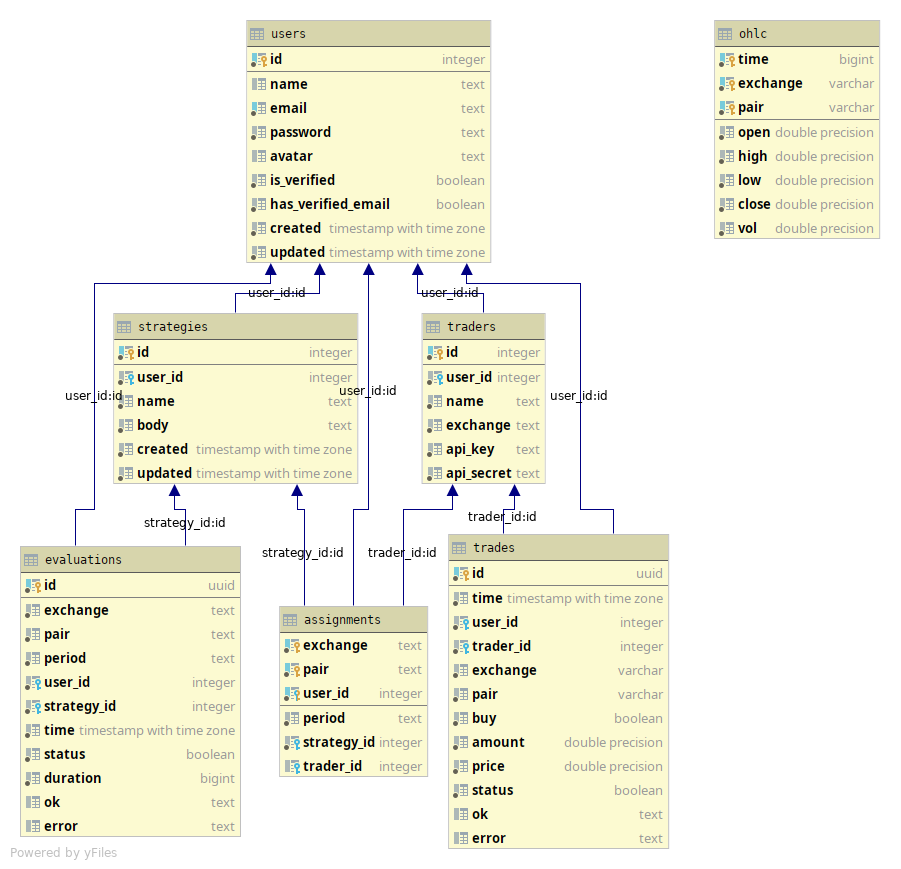
\includegraphics[width=\textwidth]{obrazky-figures/db.png}
    \caption{Database structure diagram}
    \label{img:arch}
\end{figure}


\subsubsection{Database access}
The access to the database, is implemented by the \verb|db| library in the \verb|code/deps| subdirectory.
This library utilizes the \verb|diesel| library
to access the database and generate queries. We could call this library an ORM(Object-Relational Mapper).
However, it operates on a lower level than most ORM solutions.

One drawback of diesel is the inherently synchronous nature of database adapters provided by this library.
In order for this component to effectively work with other components, we first must provide an asynchronous interface
to the database. There are 2 key techniques we utilize.

First of all, each component does not have only one connection to the database, We utilize the \verb|r2d2| library
to create a pool of reusable connections. Then, in order to execute queries concurrently, we run database queries
in dedicated actors. These actors utilize Actix's \textbf{SyncContext} instead of normal \textbf{Context}. The main difference
is that when using \textbf{SyncContext}, each actor runs in separate thread, and runs synchronously, while responding to
messages with asynchronous \textbf{Futures}. Each component runs at least 4 of these actors.

For ease of development, we created the \textbf{Database} struct, that encapsulates all this behavior, and provides
a set of asynchronous methods, which implement required actions. Most of these method implement common actions
from the CRUD pattern (Create-Read-update-Delete), which creates a lot of redundancy. We aim to reduce this redundancy
by implementing generic \textbf{Repository} pattern. However, due to diesel's heavy use of complex traits, we
were unable to do so within this thesis' time frame.

\subsection{Web component}
This system component implements the REST API necessary to access the system. This API is then
in turn used by the frontend web application. In theory, this API could be published for consumption by
other developers that wish to extend our system.

The API is implemented using the \verb|actix-web| library, that utilizes the actor model to its fullest,
being one of the fastest HTTP library in the world\cite{techempower_benchmark}. This library
allows programmer to attach individual functions to HTTP URIs, and these functions are then invoked by a
set of worker actors, whenever they receive a request matching said URI. The library also performs automatic parsing
of path and query parameters and request bodies. Another core part of the library interface is the programmer defined
state, that can be attached to a running web server. This state can be then retrieved inside every handler function.

Our implementation uses it to store handle to database access actors, which are then used for retrieving data.
This is implemented using the \textbf{Database} wrapper struct, that was described earlier.

Most of the implemented endpoints act as a simple interface to the database, that performs some validation, but there
are some custom logic.

This part of the system heavily relies upon the async-await style of programming, that requires the nightly compiler.
Every single handler method is implemented as an async function which internally calls several other async functions.

%@formatter:off
\begin{code}[language=rust,label={web_handler},caption={Example web handler function}]
async fn api_detail((req, id): (HttpRequest, Path<i32>)) -> Result<impl Responder> {
    let db: Database = base.state.db.clone();
    let base = await_compat!(BaseReqInfo::from_request(&req))?;
    require_login!(base);

    let (strat, user) = await_compat!(db.strategy_data(id.into_inner()))?;
    let evals = await_compat!(db.get_evals(strat.id))?;
    require_cond!(strat.user_id == base.auth.uid, "Not authorized");

    Ok(Json(strat).respond_to(&req).unwrap())
}
\end{code}
%@formatter:on

The \autoref{web_handler} code sample shows an example of a handler method, that is used for retrieving a strategy from the database.
First important aspect is the method argument, which is a tuple of the request and a path parameter, that is automatically extracted by
the library.

The function first clones a handle to the database wrapper, and then retrieves basic info from the request.
The \textbf{BaseReqInfo} struct primarily contains the authorization information. This retrieval must be asynchronous,
since it might require a database access. This asynchronous operation is then wrapped in a \verb|await_compat| macro, which internally wraps
the \verb|await| macro.

Then, the strategy is retrieved from database, and \verb|require_cond| macro is used for ensuring that user can only access strategies that he owns.

Finally, the strategy is serialized wrapped in the \verb|Json| struct, that performs serialization into Json in the
\verb|respond_to| method.

\section{Web application frontend}
As mentioned earlier, the frontend application is implemented as a react single page application.
This approach was chosen after a long series of experiments with multiple approaches to web applications.

The first tried approach was completely server-side rendered site that utilizes static html forms for
submitting data. While this approach did work, the problem was extremely poor UX, and very complex generated forms that utilized hidden fields in order to preserve information
for form submission.

The completely server-side generated site was then progressively rewritten into combined
application, that used forms for submitting data, but utilized custom web components
based \verb|LitElement| library to reduce complexity and provide some amount of dynamic behavior, improving
user experience. However, there were problems with this approach too. The user experience still did not meet the
standards expected by modern users, and the application logic was now in 2 languages distributed acros 2 codebases,
greatly complicating futher development.

After both of these approaches failed, we elected to rewrite the web interface part of the system from scratch.
This time, the backend was rewritten to the form of a REST API described earlier, and the frontend application
was rewritten in React. We also decided to use Redux\footnote{https://redux.js.org/} to manage application state,
and Material-UI library to provide set of base components, foregoing any kind of complex UI template.

\subsection{React}
As mentioned earlier, React is javascript library for writing user interfaces, that utilizes custom JSX syntax.
The web applciation code resides in \verb|code/web/app| and during compilation of the web component, the
compiled web application is bundled inside the \verb|web| binary using \verb|includeddir| library.

This web applicaiton is then provided on the \verb|/app| prefixed URI routes, while the \verb|api| prefix
contains all the REST endoints. The web server provides the same \verb|index.html| page for every subroute under
the \verb|app| prefix, and this generated index file imports resources from the \verb|/static| prefix, that
refers to individual files of compiled react application.

\subsection{Components \& Routing}
The application is divided into several root components, each root component roughly corresponding to single
'page' of the application. Because the server provides \verb|index.html| for every URI under the \verb|/app| prefix, the
routing between indivudual components that reside under this prefix is performed in the browser using the
\verb|react-router| library. This library switches rendered component based on current path.
Follwoing example shows the JSX for the root of the application.

%@formatter:off
\begin{code}[language=html,label={react_routing},caption={React application routing JSX}]
<div className="App">
    <ConnectedRouter history={history}>
        <Switch>
            <Route exact path="/app/auth" component={Login}/>
            <Route path="/app" render={props => (
                <Dashboard>
                    <Switch>
                        <Route exact path="/app/" component={Home}/>
                        <Route exact path="/app/strategies" component={StrategyList}/>
                        <Route exact path="/app/strategies/:id" component={StrategyDetail}/>
                        <Route exact path="/app/assignments" component={AssignmentList}/>
                        <Route exact path="/app/traders" component={TraderList}/>
                    </Switch>
                </Dashboard>
            )}/>
        </Switch>
    </ConnectedRouter>
</div>
\end{code}
%@formatter:on

\subsubsection{Dashboard}
This component contains the base layout of the web application, rendering the toolbar with title, navigation bar,
and also rendering nested components. In our case, the nested component is the react-router \textbf{Switch},
that ensures only one route from a set of route elements is active at one time. This \textbf{Switch} component
with the set of inner routes contains the individual pages.

\subsection{Redux}
Another important aspect of the web application was the storage, and management of state. The earlier attempts failed
because the management of state was untenable with growing application complexity.
the \verb|Redux| library was developed precisely to solve this problem.
As described earlier, the library is based on the \textbf{Flow} architecture pattern, which has 3 core concepts.

\begin{figure}[H]
    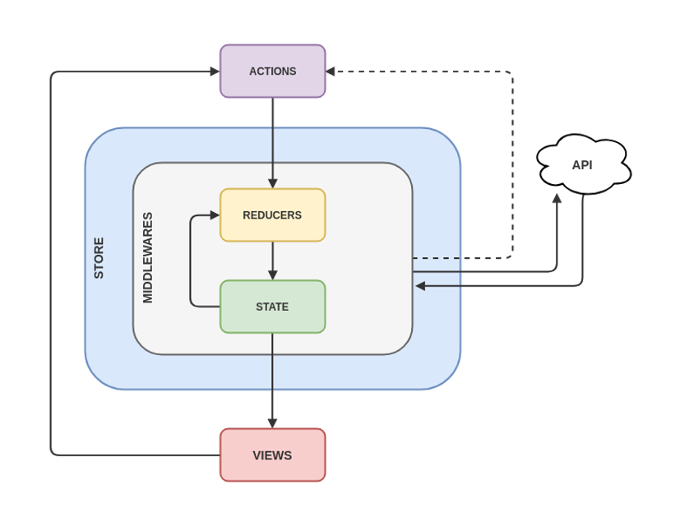
\includegraphics[width=\textwidth]{obrazky-figures/redux.png}
    \caption{Redux general diagram}
    \label{img:redux}
\end{figure}


The redux store contains the application state, and is only mutable inside reducers. The redux reducers are used
to modify state, based on the actions,that are published by components, and the components then in turn react to
changes of state.


Our usage of redux creates the state upon application creation, along with a single reducer which is responsible
for storing data received from the REST API inside this state. The access to the REST API is implemented in
\verb|api/baseApi.js| file. This file contains a metadata object for each entity exposed by the API, and
a \verb|Api| class that contains methods for executing common methods.

However, this class is not used directly, its only used from the \verb|actions/apiActions.js| file, that
provides methods for contacting the API and then dispatching the results as redux actions. It utilizes
the \verb|redux-thunk| middleware.

These actions are then processed by the \verb|dataReducer|, which is responsible for reflecting the changes inside the
data store. First versions did so manually, but the growing complexity forced us to adopt the \verb|Redux-ORM| library.
This library provided simple ORM-like experience, and definitely made the development easier.

\subsection{Material-UI}
This library was chosen as a base library of components, upon which our custom components were built.
It implements commonly needed components that conform to Google's Material design guidelines\footnote{https://material.io/design/}.
These components are also written with first class support of mobile devices, opening up the pathway for
making our web application into a Progressive Web Application\footnote{https://en.wikipedia.org/wiki/Progressive\_web\_applications}.

Core component used in our custom components is the \verb|Paper| component, which creates a surface
with the appearance of an elevated piece of paper. This concept of an elevated surface is also at the core of
Material design guidelines.

Each custom component is implemented as a list of these \verb|Paper| surfaces, each one holding some kind of information.
Most commonly, these surfaces contains tables that show existing entities of a given type, along with a button to add new entity.

\subsubsection{EditDialog}
The creation and editing of data entities is performed by editing a set of fields inside a modal dialog containing a
form. During development, this pattern of a modal dialog with form organically appeared at multiple points, and therefore we decided to implement a
single component that would replace individual forms.

This resulted in the implementation of \textbf{EditDialog} react component, which performs editing of a javascript object according
to properties passed into it.

%@formatter:off
\begin{code}[language=html,label={edit_dialog},caption={EditDialog for creation of Trader account}]
<EditDialog
    open={this.state.open}
    data={this.state.newTrader}
    title="New trader"
    text="Create a new trading account"
    onData={(d) => {
        this.setState({newTrader: d})
    }}
    attrs={[
        {name: "name", title: "Name", type: "text"},
        {name: "api_key", title: "Api key", type: "text"},
        {name: "api_secret", title: "Api secret", type: "text"},
        {name: "exchange", title: "Exchange", type: "select", values: values, text: (e) => e}
    ]}
    onDismiss={(save) => {
        this.setState({open: false});
        if (save) {
            dispatch(postOne(TYPE_TRADER, this.state.newTrader)).then(() => {
                this.setState({open: false});
            })
        }
    }}
/>
\end{code}
%@formatter:on

The \autoref{edit_dialog} contains code for rendering an \textbf{EditDialog}, that performs creation of new trader
account. It uses data-binding to to pass properties, and callback functions into the dialog.
\begin{itemize}
    \item {open -} Whether the dialog is shown or hidden
    \item {data - } Data object for editing
    \item {title - } Title of the dialog
    \item {text - } Information text of the dialog
    \item {onData - } Callback function that receives changed object
    \item {attrs - } A list of attributes, that should be mapped to editable fields
    \item {onDismiss - } Callback function invoked when dialog is dismissed, receives whether the dismissal was performed
    by the OK button or otherwise.
\end{itemize}


\chapter{Testing and evaluation}
This chapter aims to describe the methodology that was used for evaluating the implemented system, and project results
as a whole. Another goal is to outline authors experience with the used technologies, and provide some guidelines for future
projects of this type.

\section{Testing}
While 2 primary implementation languages of this project (Rust + React Javascript) have excellent support for unit testing,
this approach for ensuring software correctness was used in minimal capacity.

To properly test the individual components and ensure their correct behavior, another approach was chosen. because of the
fact, that the project uses kubernetes for management, and deployment of the implemented system, allowed us to create
separate testing environment. The system was then primarily deployed into this environment, and was observed.
This approach allowed us to observe the system in virtually the same environment, in which it will be deployed.
Several complex behaviors arisen from interaction of individual components were observed, and subsequently fixed.
We wouldn't be able to observe these issues without all the components integrated together, so subjectively, we
feel that the chosen approach was correct.

\subsubsection{Example case - Silent disconnects}
One of the observed complex interaction behaviors was the problem of long-lived connections in the environment, in
which components are removed and added dynamically.
The ZeroMQ library has a complex internal networking layer, that utilizes several sockets, and a separate thread
for managing them.

Our \verb|actix_net| uses ZeroMQ, and uses several different virtual socket types provided by it. These sockets
are long-lived. They should stay open during the whole time the component runs. However, in the kubernetes environment,
components can be killed at virtually any time. This poses a problem. For Router and PUB socket types that were
used in \actor{ServiceHandler} and \actor{Publisher} actors respectively, the ZeroMQ library does not detect disconnects, or detects
them after some time.

This duration between disconnect and detection of it caused an issue with a large amount of missed messages, which
destabilized the whole system. The component that was affected the most, was the \actor{Ingest} actor in the \kubecomp{core}
component, which could not detect missing OHLC updates, since it was a binding SUB socket that created a SUB topology.

The approach, that we chose to fix this issue was to use features of the TCP protocol implementation know as Keepalive.
This feature is so called, because it can be usd to keep a TCP connection alive and well, and determine when it was dropped from the other side.

The primary mechanism for performing this service is to periodically send empty TCP packets, that must be acknowledged from
the other side. If a sequence of packets is not acknowledged in some pre-defined time, the connection is considered cloesd
from the other side, and is dropped. Usage of this feature required the modification of \verb|tokio-zmq| library, that provides
asynchronous implementation
of ZeroMQ sockets. This change allowed setting custom options on the underlying sockets.

\subsection{Debugging}
However, sometimes it was necessary to observe the internal state of a particular component while it is integrated in the system.
Initially, this provided to b quite a difficult challenge, since kubernetes utilizes containers, and accessing the container
internals is difficult.

But, after some research, we discovered the Telepresence\footnote{https://www.telepresence.io/} command line tool. This tool is written in python,
and it creates a vpn tunnel to a container that is running in the kubernetes cluster. Allowing local applications to run as if
the were ran inside the actual kubernetes environment.

The fact that we could now run individual components locally, with a debugger greatly simplified the testing and bug fixing process.

\subsection{Monitoring}
Another important aspect was the monitoring of deployed system, with particular emphasis put upon
the monitoring of system performance, and access to individual container logs.

At first, we only used the \verb|kubectl| command line tool. But during during the development the system kept growing
in size, and with it the number of components that needed to be monitored has grown too. We solved this issue by installing

a Kubernetes Dashboard\footnote{https://github.com/kubernetes/dashboard} into our cluster, and using this dashboard for monitoring, visualization and log access.

Currently, we use only the metrics provided by kubernetes dashboard out of the box, but in the future, we might export
custom metrics specific to our application, that would allow us to better understand the internal system status.

\section{Implementation evaluation}
The need for low latency, scalability and predictable performance was one of the driving forces for multiple key decisions in this project.
The implementation language, communication technology, deployment strategy were all chosen in order to achieve these goals.
This section aims to evaluate, whether we achieved these goals.

\subsection{Measurement methodology}
In order to precisely measure key aspects of the implementation, the system had to be modified. the primary change
is addition of a \verb|Measurement| component in the system, that receives data from other components and holds the
"global" clock. Because of the distributed nature, the true global clock does not exist, but using a component that
will utilize its internal clock to annotate events in the system should provide enough precision for our purposes, since
we are measuring on the scale of milliseconds.

\subsubsection{Latency measurements}
First step to allow for measuring latency is annotating a data update with unique identifier, which will be passed on throughout the system.
The components will the use this identifier to uniquely identify all messages associated with a particular update.
Then, throughout normal system function, each component in the system will send messages denoting the state of a particular message along with its identifier
to measuring component. This approach might add some latency, but considering that several of the processing steps
take several milliseconds, it should be precise enough for our purposes.

\subsubsection{Scalability measurements}
The scalability measurement is closely associated with the latency measurement. We measured the scalability of the system
by adding virtual strategies and corresponding assignments to the system, increasing the load put upon it. Then , we measured,
how the system latency was affected. With the increase in computing requirements, the computing resources
available to the kubernetes cluster were also increased.

\section{Performance measurements}
The performance measurements were taken in production environment. We utilized custom component described earlier. This component aggregated
messages from all other components, marking each event with the timestamp, the moment it was received. Then, periodically, this
data was processed in memory, and written into a CSV file, that was then copied from the docker container this component was
running inside. After obtaining the measured data, some basic statistical analysis was performed.

\subsection{Collected information}
Since the core metrics we are interested in are the individual latencies. We collect latencies of individual steps locally, and
aggregate the results on the \actor{Measure} component. The data was collected using several configurations and system loads.
These configurations are:

\begin{table}[H]
    \centering
    \addtolength{\leftskip} {-2cm}
    \addtolength{\rightskip}{-2cm}
    % Please add the following required packages to your document preamble:
    % \usepackage{multirow}
    \begin{tabular}{|l|l|l|l|l|l|l|l|l|}
        \hline
        \multirow{2}{*}{Config} & \multicolumn{2}{l|}{Nodes}                                     & \multirow{2}{*}{Core}                                     & \multirow{2}{*}{Postgres}                                 & \multirow{2}{*}{Balancer}                                 & \multicolumn{2}{l|}{Workers}                                                    & \multirow{2}{*}{Price} \\ \cline{2-3} \cline{7-8}
        & \# & Type & & & & \# & Type &                        \\ \hline
        C1 & 2 & \begin{tabular}[c]{@{}l@{}}
                     2 vCPU\\ 2 GB RAM
        \end{tabular} & \begin{tabular}[c]{@{}l@{}}
                            100 mCPU\\ 100 MB
        \end{tabular} & \begin{tabular}[c]{@{}l@{}}
                            500 mCPU\\ 500 MB
        \end{tabular} & \begin{tabular}[c]{@{}l@{}}
                            200 mCPU\\ 100 MB
        \end{tabular} & 3 & \multirow{2}{*}{\begin{tabular}[c]{@{}l@{}}
                                                300 mCPU\\ 150 MB
        \end{tabular}} & \$ 30                  \\ \cline{1-7} \cline{9-9}
        C2 & 4 & \begin{tabular}[c]{@{}l@{}}
                     2 vCPU\\ 2 GB RAM
        \end{tabular} & \begin{tabular}[c]{@{}l@{}}
                            200 mCPU\\ 100 MB
        \end{tabular} & \begin{tabular}[c]{@{}l@{}}
                            1.5 CPU\\ 1.5 GB
        \end{tabular}  & \begin{tabular}[c]{@{}l@{}}
                             400 mCPU\\ 100 MB
        \end{tabular} & 8 & & \$ 60                  \\ \hline
    \end{tabular}
\end{table}


As you can see, we started with a simple configuration utilizing 2 nodes, and limiting resources available to individual components. Then,
as we increased load put upon the system, we increased the number of nodes, and increased resources available to individual components
accordingly.

\subsubsection{Strategy}
The strategy used for testing is the following:


%@formatter:off
\begin{code}[language={[5.2]Lua},label={test_strategy},caption={Example strategy}]
-- Fast exponential moving average closely follows price while smoothing out
-- random swings
local ema_fast = ta.ema(3)
-- Slow exponential moving average tracks longer term trend
local ema_slow = ta.ema(29)

-- We use RSI to determine when an asset is overbought or oversold
local rsi = ta.rsi(14)

-- Triggering signal for buying and selling
local buy_signal = ema_fast() > ema_slow() * 1.001
local sell_signal = ema_fast() < ema_slow() * 0.999

-- RSA guards for overbought or oversold markets
local rsi_overbought = rsi() > 80
local rsi_oversold = rsi() < 20

if buy_signal and not rsi_overbought then
    return 'long'
elseif sell_signal and not rsi_oversold then
    return 'short'
else
    return 'neutral'
end
\end{code}
%@formatter:on


This simple strategy utilizes 3 indicators from \verb|ta| library, applied to different timeframes of data, and
performs some arithmetic operations to determine the state of the market. For measurement purposes, we removed foreign key
constraints from the database, and used this strategy for numerous virtual users.
\newpage

\section{Results}
After performing several test runs, we measured the latency of the some parts of the system, and also the global system
latency. These measurements were then performed for different configurations and different amount of load put upon the system.

\begin{figure}[H]
    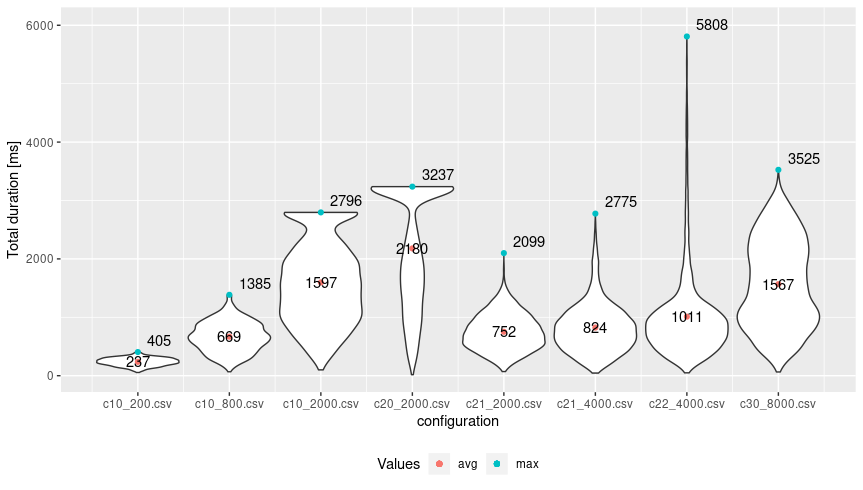
\includegraphics[width=\textwidth]{obrazky-figures/agg.png}
    \caption{Aggregate performance measurements}
    \label{img:measure_agg}
\end{figure}

The \autoref{img:measure_agg} shows measured latencies for data passing through whole system for multiple configurations and
number of assignments. The x axis stands for specific measurement, and the Y axis shows latency of the system. The graph
also contains values of average and maximum latencies measured.


We tested 2 system configurations. In the first, configuration, the system was able to preserve total system latency below
1 second for 99 \% of cases with at most 4000 assignments. In second configuration, the system was able to preserve this latency
when serving at most 16 000 assignments. Considering the target audience, it is very unlikely, this particular system
will ever see utilization this high.


\subsection{Measurement stages}
However, we were not able to achieve the necessary latency when system had insufficient resources
for a specific number of assignments. To determine which part of the system
was bottleneck in which configuration, we measured different stages of the system separately.

These stages are:
\begin{itemize}
    \item{Save} - Duration of saving newly received data into the database
    \item{Dispatch} - Duration between sending a evaluation request, and worker processing this request
    \item{Load} - Duration of lading historical data from database
    \item{Exec} - Duration of actual strategy execution
\end{itemize}


\subsubsection{Specific stage measurements
}

Graphs for these stages follow:
\begin{figure}[H]
    \centering
    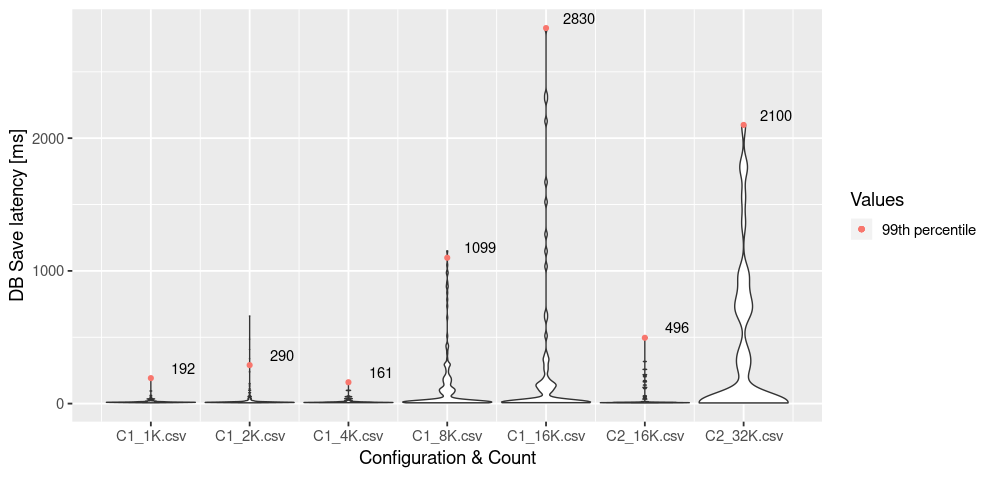
\includegraphics[width=1\textwidth]{obrazky-figures/save.png}
    \caption{Saving data performance measurements}
    \label{img:measure_save}
\end{figure}
\begin{figure}[H]
    \centering
    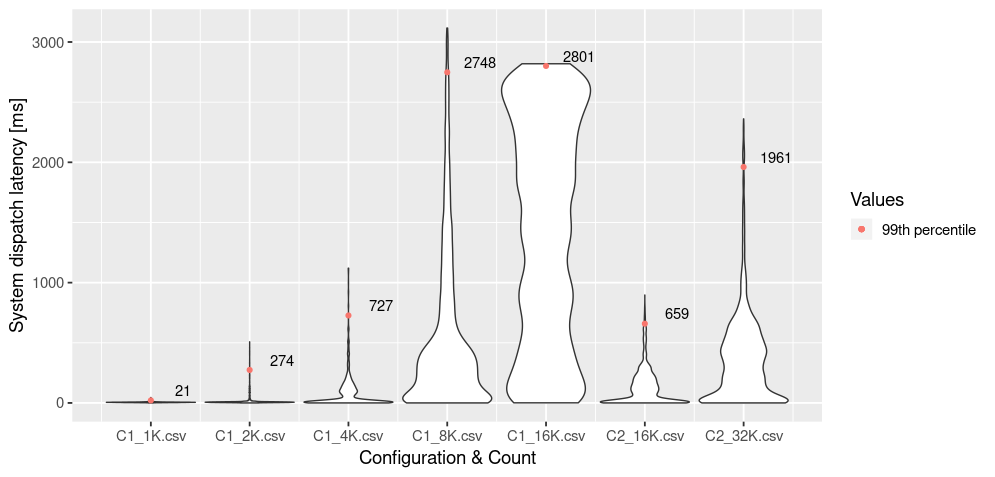
\includegraphics[width=1\textwidth]{obrazky-figures/dispatch.png}
    \caption{Data dispatch performance measurements}
    \label{img:measure_dispatch}
\end{figure}

\begin{figure}[H]
    \centering
    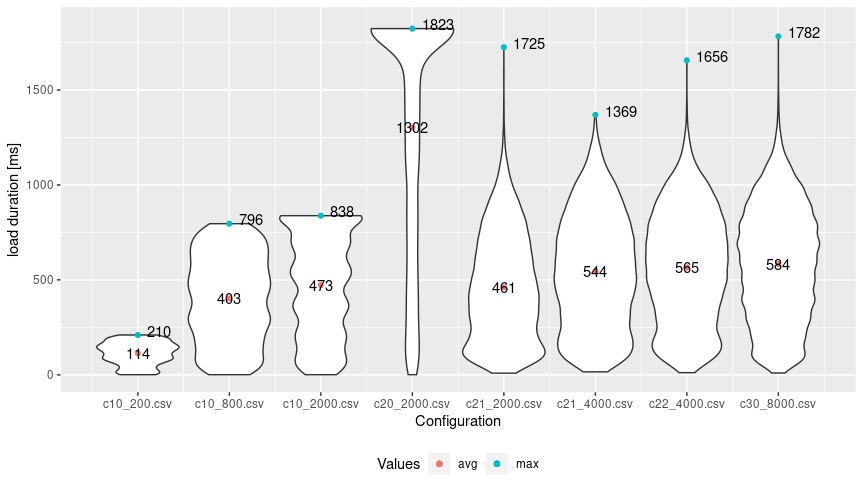
\includegraphics[width=1\textwidth]{obrazky-figures/load.png}
    \caption{Loading data performance measurements}
    \label{img:measure_load}
\end{figure}


\begin{figure}[H]
    \centering
    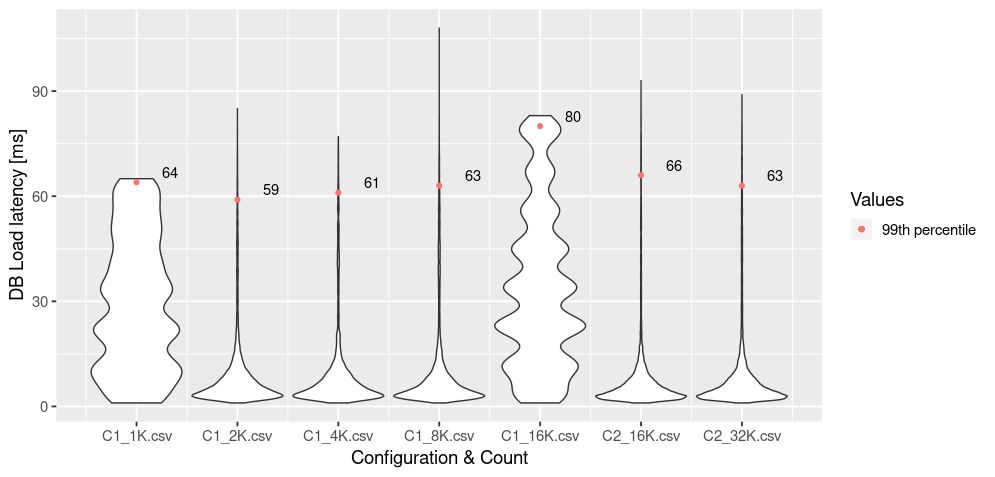
\includegraphics[width=1\textwidth]{obrazky-figures/exec.png}
    \caption{Execution performance measurements}
    \label{img:measure_exec}
\end{figure}


If we examine these graphs in detail, we can discern how configuration changes affected the system.
In each configuration, the load and execute stages latencies had stayed relatively stable.

\subsubsection{C1}
In first configuration, the system was able to support at most 4000 assignments. When the system load
exceeded this number, the time spent in the dispatch stage had risen considerably. This points to an issue with
not enough workers evaluating strategies.

\subsubsection{C2}
In second configuration, the system was able to support 16000 assignments seamlessly however, when system had to
serve 32000 assignments, the database subsystem was unable to handle the load, and the time required to save
incoming data into the database has risen considerably. This increase in latency was certainly a result of
increased general database load.

\subsection{Further scaling}
We performed some experimental testing with even larger configurations and assignment counts up to 128 thousand,
but, due to limited time, we were unable to get the system into working state,since in these configurations,
the system had to service several thousand requests per second. Considering the expected system load,
we abandoned this configuration.

\subsection{Automatic scaling}
Configurations shown were created manually. This resulted in some mismatch between amount of resources available, and provided
to specific components. In the future, we plan to utilize both horizontal and vertical pod autoscaling capabilities of kubernetes
to automatically scale individual components. Along with pod autoscaling, several kubernetes implementations also provide
automatic cluster scaling. By combining these 2 tools, we could make the system totally independent, even in the event
of sudden increased or decreased load.


\section{Problems}
While we can point to many positive aspects of the system, we would be remiss, if we wouldn't take its problems
into consideration as well. Some of these problems were observed throughout the development, and some were only discovered
upon testing.

\subsection{Database bottlenecks}
When scaling the system to several thousand users, the chosen database solution seems to perform inadequately.
When faced with high loads the database is no longer able to provide historical data for individual workers fast enough.
This, in turn slows down dispatching of new requests since existing workers are busy loading data from database, and therefore the
load balancing component must wait for new workers to become available. The actual strategy execution stage has relatively
stable latency.

To solve this problem, we will have to increase the number of available workers even further, and introduce some kind of
local cache for historical data that would reduce the database pressure.

\subsection{Readability problems}
While most of the implementation benefited greatly from the use of Rust as primary implementation language, the combination
of this language, with its very explicit asynchronous style of coding resulted in some sections of the code being
very hard to read, and therefore understand. We hope, that this drawback is resolved by full migration
to async-await style programming upon its stabilization within the language.

The system as a whole probably requires a refactoring pass, since it was developed over the course of a year,
and some decisions taken at the beginning proved to be wrong, and the system had to be adapted.

\subsection{Deployment updates - Disconnects}
As mentioned in our overview of system testing, the individual components of the system suffered from silent disconnects.
While this issue was mostly resolved, it points to a much deeper issue with the use of ZeroMQ as a transport technology.
It requires management. If we have used simple HTTP based REST api to communicate between components, the disconnections
would have resulted in individual call failures almost immediately, greatly reducing the instability of the system during
an upgrade.

However, we hope to fix this issue, by adding multiple ZeroMQ sockets to single communication actor, with some
of them being used for sending heartbeats and therefore detecting network or component failures.

\section{Impact of selected technologies}
Due to design constraints, we have elected to use rather uncommon set of technologies. Now, after measuring system
performance, we can evaluate, how these choices affected our results

\subsubsection{ZeroMQ}
We elected to use ZeroMQ instead of using raw TCP sockets or higher level approach of using HTTP.
This choice brought low latency messaging, which ultimately was overshadowed by general system latency. However, the
different socket types proved useful for implementing custom communication patterns. Ultimately, we
believe, that the choice of ZeroMQ was a right one, and in the future, when the system is more optimized, its benefits
will overshadow the initial difficulties encountered.

\subsubsection{Rust}
The choice of Rust for main implementation language was primarily influenced by availability of very good library
implementing The actor model (Actix), low overhead and primitives for asynchronous programming. Thanks to the
use of this language, all components of the system require very low amounts of RAM, most of which
is consumed by kubernetes. The use of Actix somewhat reduced the readability of code, but allowed us to create
fully asynchronous components, which increased system throughput considerably.

Overall, we regard this choice as a good one. With some updates to the language which should be available soon (Await syntax)
we should be able to increase the readability of the code, while preserving all the benefits.

\subsubsection{Lua}
Based on measurements we collected over large amount of strategy executions, we can safely say, that the implementation
of strategies in LUA was a good choice. The evaluation workers have shown very stable latency, and thanks to the use of this language,
we were able to create a sandbox, securing the system from this attack vector.

\subsubsection{Postgres}
And finally, the choice of PostgreSQL with TimescaleDB for storing asset data. In the beginning of this project, this choice vas very attractive,
since it allowed us to use single database for System and asset data, greatly reducing complexity of the system.
This choice provided adequate performance throughout the development of the system.

However, when testing the system with a significant load, the asset data storage solution proved to be inadequate, being
one of the main bottlenecks, reducing system latency. Through configuration changes, we were able to tune the database. These
changes allowed us to serve around than 16000 assignments with acceptable latency.

However, if the system gains more users, we will have to change the storage solution, or provide some caching mechanisms,
to reduce database pressure.

Overall, we regard this choice as not very good one, and in the future, we would generally choose a different approach(probably
scyllaDB) for these kinds of storage requirements.

\chapter{Conclusion \& Future work}
The aim of this thesis was design and creation of a distributed system with with very specific constraints.
These constraints aimed our approach to the system, and affected our choice of technologies.

The system was implemented as a distributed application with a Single-page application as web frontend. We utilized
ZeroMQ for communication, and based the general system architecture on the actor model.

As part of this thesis, we have designed and implemented 2 libraries (\verb|actix-comm| and \verb|actix-net|), which
will released as open-source into the Actix library ecosystem.

We measured the performance achieved by the system depending on the load being put on it, and its ability to scale to
utilize more computational resources in accordance with the rise in system load.

The system designed was submitted into the Excel@FIT student conference. The feedback provided by attendees of this
conference was invaluable, and will certainly influence the future of the system.

While we feel we successfully satisfied all the requirements put forward in the initial stages of this thesis,
we feel that both the set of technologies chosen, and the implemented system have bigger potential, than was
realized. We aim to explore this unrealized potential even after this thesis is finished by continued development,
and eventual release of the implemented system as a fully functional service.


\section*{Future Work}
The system created during the course of this thesis is currently deployed, and available to users.
To fully realize capabilities of the system, we aim to improve it in several ways.

First, we will focus on the usability of the system, improving the frontend application, and creating some kind of
tutorial. Then after the system is ready to be released, we hope to get some feedback from real users, and
focus on areas determined by the feedback.

From the system side, we aim to clean up the code of the \verb|actix-net| and \verb|actix-arch| libraries,
and release them in the crates.io ecosystem.


  
  % Kompilace po částech (viz výše, nutno odkomentovat)
  % Compilation piecewise (see above, it is necessary to uncomment it)
  %\subfile{projekt-01-uvod-introduction}
  % ...
  %\subfile{chapters/projekt-05-conclusion}


  % Pouzita literatura / Bibliography
  % ----------------------------------------------
\ifslovak
  \makeatletter
  \def\@openbib@code{\addcontentsline{toc}{chapter}{Literatúra}}
  \makeatother
  \bibliographystyle{bib-styles/slovakiso}
\else
  \ifczech
    \makeatletter
    \def\@openbib@code{\addcontentsline{toc}{chapter}{Literatura}}
    \makeatother
    \bibliographystyle{bib-styles/czechiso}
  \else 
    \makeatletter
    \def\@openbib@code{\addcontentsline{toc}{chapter}{Bibliography}}
    \makeatother
    \bibliographystyle{bib-styles/englishiso}
  %  \bibliographystyle{alpha}
  \fi
\fi
  \begin{flushleft}
  \bibliography{projekt-20-literatura-bibliography}
  \end{flushleft}

  % vynechani stranky v oboustrannem rezimu
  % Skip the page in the two-sided mode
  \iftwoside
    \cleardoublepage
  \fi

  % Prilohy / Appendices
  % ---------------------------------------------
  \appendix
\ifczech
  \renewcommand{\appendixpagename}{Přílohy}
  \renewcommand{\appendixtocname}{Přílohy}
  \renewcommand{\appendixname}{Příloha}
\fi
\ifslovak
  \renewcommand{\appendixpagename}{Prílohy}
  \renewcommand{\appendixtocname}{Prílohy}
  \renewcommand{\appendixname}{Príloha}
\fi
%  \appendixpage

% vynechani stranky v oboustrannem rezimu
% Skip the page in the two-sided mode
%\iftwoside
%  \cleardoublepage
%\fi
  
\ifslovak
%  \section*{Zoznam príloh}
%  \addcontentsline{toc}{section}{Zoznam príloh}
\else
  \ifczech
%    \section*{Seznam příloh}
%    \addcontentsline{toc}{section}{Seznam příloh}
  \else
%    \section*{List of Appendices}
%    \addcontentsline{toc}{section}{List of Appendices}
  \fi
\fi
  \startcontents[chapters]
  \setlength{\parskip}{0pt}
  % seznam příloh / list of appendices
  % \printcontents[chapters]{l}{0}{\setcounter{tocdepth}{2}}
  
  \ifODSAZ
    \setlength{\parskip}{0.5\bigskipamount}
  \else
    \setlength{\parskip}{0pt}
  \fi
  
  % vynechani stranky v oboustrannem rezimu
  \iftwoside
    \cleardoublepage
  \fi
  
  % Přílohy / Appendices
  % Tento soubor nahraďte vlastním souborem s přílohami (nadpisy níže jsou pouze pro příklad)
% This file should be replaced with your file with an appendices (headings below are examples only)

% Umístění obsahu paměťového média do příloh je vhodné konzultovat s vedoucím
% Placing of table of contents of the memory media here should be consulted with a supervisor
%\chapter{Obsah přiloženého paměťového média}

%\chapter{Manuál}

%\chapter{Konfigurační soubor} % Configuration file

%\chapter{RelaxNG Schéma konfiguračního souboru} % Scheme of RelaxNG configuration file

%\chapter{Plakát} % poster

\chapter{Jak pracovat s touto šablonou}
\label{jak}

V této příloze je uveden popis jednotlivých částí šablony, po kterém následuje stručný návod, jak s touto šablonou pracovat. Pokud po jejím přečtení k šabloně budete mít nějaké dotazy, připomínky apod., neváhejte a napište na e-mail sablona@fit.vutbr.cz.

\section*{Popis částí šablony}

Po rozbalení šablony naleznete následující soubory a adresáře:
\begin{DESCRIPTION}
  \item [bib-styles] Styly literatury (viz níže). 
  \item [obrazky-figures] Adresář pro Vaše obrázky. Nyní obsahuje placeholder.pdf (tzv. TODO obrázek, který lze použít jako pomůcku při tvorbě technické zprávy), který se s prací neodevzdává. Název adresáře je vhodné zkrátit, aby byl jen ve zvoleném jazyce.
  \item [template-fig] Obrázky šablony (znak VUT).
  \item [fitthesis.cls] Šablona (definice vzhledu).
  \item [Makefile] Makefile pro překlad, počítání normostran, sbalení apod. (viz níže).
  \item [projekt-01-kapitoly-chapters.tex] Soubor pro Váš text (obsah nahraďte).
  \item [projekt-20-literatura-bibliography.bib] Seznam literatury (viz níže).
  \item [projekt-30-prilohy-appendices.tex] Soubor pro přílohy (obsah nahraďte).
  \item [projekt.tex] Hlavní soubor práce -- definice formálních částí.
\end{DESCRIPTION}

Výchozí styl literatury (czechiso) je od Ing. Martínka, přičemž slovenská a anglická verze (slovakiso a englishiso) jsou jeho překlady s drobnými modifikacemi. Oproti normě jsou v~něm určité odlišnosti, ale na FIT je dlouhodobě akceptován. Alternativně můžete využít styl od Ing. Radima Loskota nebo od Ing. Radka Pyšného\footnote{BP Ing. Radka Pyšného \url{http://www.fit.vutbr.cz/study/DP/BP.php?id=7848}}. Alternativní styly obsahují určitá vylepšení, ale zatím nebyly řádně otestovány větším množstvím uživatelů. Lze je považovat za beta verze pro zájemce, kteří svoji práci chtějí mít dokonalou do detailů a neváhají si nastudovat detaily správného formátování citací, aby si mohli ověřit, že je vysázený výsledek v pořádku.

\begin{samepage}
Makefile kromě překladu do PDF nabízí i další funkce:
\begin{itemize}
  \item přejmenování souborů (viz níže),
  \item počítání normostran,
  \item spuštění vlny pro doplnění nezlomitelných mezer,
  \item sbalení výsledku pro odeslání vedoucímu ke kontrole (zkontrolujte, zda sbalí všechny Vámi přidané soubory, a případně doplňte).
\end{itemize}
\end{samepage}

Nezapomeňte, že vlna neřeší všechny nezlomitelné mezery. Vždy je třeba manuální kontrola, zda na konci řádku nezůstalo něco nevhodného -- viz Internetová jazyková příručka\footnote{Internetová jazyková příručka \url{http://prirucka.ujc.cas.cz/?id=880}}.

\paragraph {Pozor na číslování stránek!} Pokud má obsah 2 strany a na 2. jsou jen \uv{Přílohy} a~\uv{Seznam příloh} (ale žádná příloha tam není), z nějakého důvodu se posune číslování stránek o 1 (obsah \uv{nesedí}). Stejný efekt má, když je na 2. či 3. stránce obsahu jen \uv{Literatura} a~je možné, že tohoto problému lze dosáhnout i jinak. Řešení je několik (od~úpravy obsahu, přes nastavení počítadla až po sofistikovanější metody). \textbf{Před odevzdáním proto vždy překontrolujte číslování stran!}


\section*{Doporučený postup práce se šablonou}

\begin{enumerate}
  \item \textbf{Zkontrolujte, zda máte aktuální verzi šablony.} Máte-li šablonu z předchozího roku, na stránkách fakulty již může být novější verze šablony s~aktualizovanými informacemi, opravenými chybami apod.
  \item \textbf{Zvolte si jazyk}, ve kterém budete psát svoji technickou zprávu (česky, slovensky nebo anglicky) a svoji volbu konzultujte s vedoucím práce (nebyla-li dohodnuta předem). Pokud Vámi zvoleným jazykem technické zprávy není čeština, nastavte příslušný parametr šablony v souboru projekt.tex (např.: \verb|documentclass[english]{fitthesis}| a přeložte prohlášení a poděkování do~angličtiny či slovenštiny.
  \item \textbf{Přejmenujte soubory.} Po rozbalení je v šabloně soubor \texttt{projekt.tex}. Pokud jej přeložíte, vznikne PDF s technickou zprávou pojmenované \texttt{projekt.pdf}. Když vedoucímu více studentů pošle \texttt{projekt.pdf} ke kontrole, musí je pracně přejmenovávat. Proto je vždy vhodné tento soubor přejmenovat tak, aby obsahoval Váš login a (případně zkrácené) téma práce. Vyhněte se však použití mezer, diakritiky a speciálních znaků. Vhodný název může být např.: \uv{\texttt{xlogin00-Cisteni-a-extrakce-textu.tex}}. K přejmenování můžete využít i přiložený Makefile:
\begin{verbatim}
make rename NAME=xlogin00-Cisteni-a-extrakce-textu
\end{verbatim}
  \item Vyplňte požadované položky v souboru, který byl původně pojmenován \texttt{projekt.tex}, tedy typ, rok (odevzdání), název práce, svoje jméno, ústav (dle zadání), tituly a~jméno vedoucího, abstrakt, klíčová slova a další formální náležitosti.
  \item Nahraďte obsah souborů s kapitolami práce, literaturou a přílohami obsahem svojí technické zprávy. Jednotlivé přílohy či kapitoly práce může být výhodné uložit do~samostatných souborů -- rozhodnete-li se pro toto řešení, je doporučeno zachovat konvenci pro názvy souborů, přičemž za číslem bude následovat název kapitoly. 
  \item Nepotřebujete-li přílohy, zakomentujte příslušnou část v \texttt{projekt.tex} a příslušný soubor vyprázdněte či smažte. Nesnažte se prosím vymyslet nějakou neúčelnou přílohu jen proto, aby daný soubor bylo čím naplnit. Vhodnou přílohou může být obsah přiloženého paměťového média.
  \item Zadání, které si stáhnete v PDF z IS FIT (odkaz \uv{Zadání pro vložení do práce} či \uv{Thesis assignment}), uložte do souboru \texttt{zadani.pdf} a povolte jeho vložení do práce parametrem šablony v \texttt{projekt.tex} (\verb|documentclass[zadani]{fitthesis}|).
  \item Nechcete-li odkazy tisknout barevně (tedy červený obsah -- bez konzultace s vedoucím nedoporučuji), budete pro tisk vytvářet druhé PDF s tím, že nastavíte parametr šablony pro tisk: (\verb|documentclass[zadani,print]{fitthesis}|). Budete-li tisknout barevně, místo \texttt{print} použijte parametr \texttt{cprint}. Barevné logo se nesmí tisknout černobíle!
  \item Vzor desek, do kterých bude práce vyvázána, si vygenerujte v informačním systému fakulty u zadání. Pro disertační práci lze zapnout parametrem v šabloně \texttt{cover} (více naleznete v souboru \texttt{fitthesis.cls}).
  \item Nezapomeňte, že zdrojové soubory i (obě verze) PDF musíte odevzdat na CD či jiném médiu přiloženém k technické zprávě.
\end{enumerate}

Obsah práce se generuje standardním příkazem \tt \textbackslash tableofcontents \rm (zahrnut v šabloně). Přílohy jsou v něm uvedeny úmyslně.

\subsection*{Pokyny pro oboustranný tisk}
\begin{itemize}
\item \textbf{Oboustranný tisk je doporučeno konzultovat s vedoucím práce.}
\item Je-li práce tištěna oboustranně a její tloušťka je menší než tloušťka desek, nevypadá to dobře.
\item Zapíná se parametrem šablony: \verb|\documentclass[twoside]{fitthesis}|
\item Po vytištění oboustranného listu zkontrolujte, zda je při prosvícení sazební obrazec na obou stranách na stejné pozici. Méně kvalitní tiskárny s duplexní jednotkou mají často posun o 1--3 mm. Toto může být u některých tiskáren řešitelné tak, že vytisknete nejprve liché stránky, pak je dáte do stejného zásobníku a vytisknete sudé.
\item Za titulním listem, obsahem, literaturou, úvodním listem příloh, seznamem příloh a případnými dalšími seznamy je třeba nechat volnou stránku, aby následující část začínala na liché stránce (\textbackslash cleardoublepage).
\item  Konečný výsledek je nutné pečlivě překontrolovat.
\end{itemize}

\subsection*{Styl odstavců}

Odstavce se zarovnávají do bloku a pro jejich formátování existuje více metod. U papírové literatury je častá metoda s~použitím odstavcové zarážky, kdy se u~jednotlivých odstavců textu odsazuje první řádek odstavce asi o~jeden až dva čtverčíky (vždy o~stejnou, předem zvolenou hodnotu), tedy přibližně o~dvě šířky velkého písmene M základního textu. Poslední řádek předchozího odstavce a~první řádek následujícího odstavce se v~takovém případě neoddělují svislou mezerou. Proklad mezi těmito řádky je stejný jako proklad mezi řádky uvnitř odstavce. \cite{fitWeb} 

Další metodou je odsazení odstavců, které je časté u elektronické sazby textů. První řádek odstavce se při této metodě neodsazuje a mezi odstavce se vkládá vertikální mezera o~velikosti 1/2 řádku. Obě metody lze v kvalifikační práci použít, nicméně často je vhodnější druhá z uvedených metod. Metody není vhodné kombinovat.

Jeden z výše uvedených způsobů je v šabloně nastaven jako výchozí, druhý můžete zvolit parametrem šablony \uv{\tt odsaz\rm }.

\subsection*{Užitečné nástroje}
\label{nastroje}

Následující seznam není výčtem všech využitelných nástrojů. Máte-li vyzkoušený osvědčený nástroj, neváhejte jej využít. Pokud však nevíte, který nástroj si zvolit, můžete zvážit některý z následujících:

\begin{description}
	\item[\href{http://miktex.org/download}{MikTeX}] \LaTeX{} pro Windows -- distribuce s jednoduchou instalací a vynikající automatizací stahování balíčků. MikTex obsahuje i vlastní editor, ale spíše doporučuji TeXstudio.
	\item[\href{http://texstudio.sourceforge.net/}{TeXstudio}] Přenositelné opensource GUI pro \LaTeX{}.  Ctrl+klik umožňuje přepínat mezi zdrojovým textem a PDF. Má integrovanou kontrolu pravopisu\footnote{Českou kontrolu pravopisu lze doinstalovat z \url{https://extensions.openoffice.org/de/project/czech-dictionary-pack-ceske-slovniky-cs-cz}}, zvýraznění syntaxe apod. Pro jeho využití je nejprve potřeba nainstalovat MikTeX případně jinou \LaTeX ovou distribuci.
	\item[\href{http://www.winedt.com/}{WinEdt}] Ve Windows je dobrá kombinace WinEdt + MiKTeX. WinEdt je GUI pro Windows, pro jehož využití je nejprve potřeba nainstalovat \href{http://miktex.org/download}{MikTeX} či \href{http://www.tug.org/texlive/}{TeX Live}. 
	\item[\href{http://kile.sourceforge.net/}{Kile}] Editor pro desktopové prostředí KDE (Linux). Umožňuje živé zobrazení náhledu. Pro jeho využití je potřeba mít nainstalovaný \href{http://www.tug.org/texlive/}{TeX Live} a Okular. 
	\item[\href{http://jabref.sourceforge.net/download.php}{JabRef}] Pěkný a jednoduchý program v Javě pro správu souborů s bibliografií (literaturou). Není potřeba se nic učit -- poskytuje jednoduché okno a formulář pro editaci položek.
	\item[\href{https://inkscape.org/en/download/}{InkScape}] Přenositelný opensource editor vektorové grafiky (SVG i PDF). Vynikající nástroj pro tvorbu obrázků do odborného textu. Jeho ovládnutí je obtížnější, ale výsledky stojí za to.
	\item[\href{https://git-scm.com/}{GIT}] Vynikající pro týmovou spolupráci na projektech, ale může výrazně pomoci i jednomu autorovi. Umožňuje jednoduché verzování, zálohování a přenášení mezi více počítači.
	\item[\href{http://www.overleaf.com/}{Overleaf}] Online nástroj pro \LaTeX{}. Přímo zobrazuje náhled a umožňuje jednoduchou spolupráci (vedoucí může průběžně sledovat psaní práce), vyhledávání ve zdrojovém textu kliknutím do PDF, kontrolu pravopisu apod. Zdarma jej však lze využít pouze s určitými omezeními (někomu stačí na disertaci, jiný na ně může narazit i při psaní bakalářské práce) a pro dlouhé texty je pomalejší. Pro vedoucí má FIT licenci a~v~případě, že student narazí na omezení, je s pomocí vedoucího situace řešitelná.
\end{description}

Pozn.: Overleaf nepoužívá Makefile v šabloně -- aby překlad fungoval, je nutné kliknout pravým tlačítkem na \tt projekt.tex \rm a zvolit \uv{Set as Main File}.

\chapter{Psaní anglického textu}
\label{anglicky}
Tato příloha je převzata ze stránek doc. Černockého \cite{CernockyEnglish}.

Spousta lidí píše zprávy k projektům anglicky (a to je dobře!), ale dělá v nich spoustu zbytečných chyb (a to je špatně). Nejsem angličtinář, ale tento jazyk už nějakých pár let používám k psaní, čtení i komunikaci -- tato příloha obsahuje pár důležitých věcí. Pokud chcete napsat práci nebo článek opravdu 100\,\% dobře, nezbude Vám než si najmout rodilého mluvčího (a to by měl by být trochu technicky zdatný a aspoň trochu rozumět tomu, co píšete, ať to neskončí ještě hůř \ldots).

\section*{Obecně}

\begin{itemize}
  \item{Předtím, než budete sami něco psát, si přečtěte pár anglických technických článků a~zkuste si zapamatovat a získat \uv{obecný pocit}, jak se to píše.}
  \item{Používejte vždy korektor pravopisu -- zabudovaný ve Wordu, nebo v OpenOffice, pokud děláte na Linuxu, tak ISPELL a další (většina editorů pro \LaTeX{} má již kontrolu pravopisu integrovanou).}
  \item{Používejte korektor gramatiky. Nevím, jestli je nějaký dostupný na Linuxu, ale ten ve Wordu celkem slušně funguje a pokud Vám něco zelené podtrhne, je tam většinou opravdu chyba. Můžete do něj nakopírovat i zdrojový text pro \LaTeX{}, opravit, a pak uložit opět jako čistý text. Pokud používáte vim, je tam zabudovaný také a zvládne jak překlepy, tak základní gramatiku. V dokumentu \texttt{diplomka.tex} na první řádek napište: 
  \begin{verbatim}
    % vim:spelllang=en_us:spell
  \end{verbatim}
  (případně \texttt{en\_gb} pro OED angličtinu)
  \textit{Poznámka editora:} Existuje i velmi dobrý online nástroj Grammarly\footnote{\url{https://www.grammarly.com/}}, který je v základní verzi zdarma. 
  }
  \item{Online slovníky jsou dobré, ale nepoužívejte je slepě. Většinou dají více variant a ne každá je správně.}
  \item{\begin{samepage}Na vyhledávání a zjištění, co bude asi správné, můžete použít Google. Např.: nevíte, jak se řekne \uv{výhoda tohoto přístupu}. Slovník na seznam.cz dá asi 10 variant. Napište je postupně do vyhledávání na googlu:
  \begin{verbatim}
    "advantage of this approach" 1100000 hits
    "privilege of this approach" 6 hits
    "facility of this approach"  16 hits
  \end{verbatim}
  Neříkám, že je to 100\,\% správně, ale je to určité vodítko. Toto se dá použít i~na~dohledání správných spojek (třeba \uv{among two cases} nebo \uv{between two cases}?)\end{samepage}}
\end{itemize}
       
\section*{SVOMPT a shoda}

Struktura anglické věty je SVOPMT: SUBJECT VERB OBJECT MANNER PLACE TIME a přes to nejede vlak! Není volná jako v češtině. Jinak to je maximálně v nějaké divadelní hře, kde je potřeba něco zdůraznit. Hlavně podmět tam musí vždycky být, na to se často zapomíná, protože v CZ/SK může být zamlčený nebo nevyjádřený. SVOMPT platí i ve vedlejších větách!
\begin{verbatim}
  BAD: We have shown that is faster than the other function. 
  GOOD: We have shown that it is faster than the other function. 
\end{verbatim}

\noindent Shoda podmětu s přísudkem -- zní to šíleně, ale dělá se v tom spousta chyb. 

\begin{verbatim}
  he has 
  the users have 
  people were 
\end{verbatim}

\section*{Členy}

Členy v angličtině jsou noční můra a téměř nikdo z nás je nedává dobře. Základní pravidlo je, že když je něco určitého, musí předtím být \uv{the}. Členy musí být určitě u těchto spojení:
\begin{verbatim}
  the first, the second, ...
  the last
  the most (třetí stupeň přídavných jmen a príslovcí) ...
  the whole 
  the following 
  the figure, the table. 
  the left, the right - on the left pannel, from the left to the right ... 
\end{verbatim}

\noindent Naopak člen NESMÍ být, pokud používáte přesné označení obrázku, kapitoly, atd.
\begin{verbatim}
  in Figure 3.2
  in Chapter 7
  in Table 6.4
\end{verbatim}

\begin{samepage}
\noindent Pozor na \uv{a} vs. \uv{an}, řídí se to podle výslovnosti a ne podle toho, jak je slovo napsané, takže:
\begin{verbatim}
  an HMM
  an XML
  a universal model
  a user
\end{verbatim}
\end{samepage}

\section*{Slovesa}

Pozor na trpné tvary sloves -- u pravidelných je to většinou bez problémů, u nepravidelných často špatně, typicky
\begin{verbatim}
  packet was sent (ne send)
  approach was chosen (ne choosed)
\end{verbatim}
\noindent \ldots vetšinou to opraví korektor pravopisu, ale někdy ne. 

Pozor na časy, občas je v nich pěkný nepořádek. Pokud něco nějak obecně je, přítomný čas. Pokud jste něco udělali, minulý. Pokud to dalo nějaký výsledek a ten výsledek teď existuje a třeba ho nějak diskutujete, přítomný. Nepoužívejte příliš složité časy jako je předpřítomný a vůbec ne předminulý pokud nevíte přesně, co děláte.
\begin{verbatim}
  JFA is a technique that works for everyone in speaker recognition. 
  We implemented it according to Kenny's recipe in \cite{Kenny}. 
  12000 segments from NIST SRE 2006 were processed. When compared 
  with a GMM baseline, the results are completely bad. 
\end{verbatim}

\section*{Délka vět a struktura}

\begin{itemize}
  \item{Pište kratší věty a souvětí, pokud máte něco na 5 řádku, většinou se to nedá číst.}
  \item{Strukturujte věty pomocí čárek (více než v češtině!), hlavně po úvodu věty, po kterém začíná vlastní věta. Někdy se dává čárka i před \uv{and} (na rozdíl od češtiny)}
\end{itemize}
\begin{verbatim}
  In this chapter, we will investigate ... 
  The first technique did not work, the second did not work as well, 
  and the third one also did not work. 
\end{verbatim}

\section*{Specifika technického textu}

Píšete technicky text, proto nepoužívejte zkratky
\begin{verbatim}
  he's
  gonna
  Petr's working on ...
\end{verbatim}
\noindent a podobně. Jediné, které je tolerované, je \uv{doesn't}, ale neuděláte chybu, když napíšete \uv{does not}. 

\begin{samepage}
\noindent V technických textech se spíš používá trpný rod než činný: 
\begin{verbatim}
  BAD: In this chapter, I describe used programming languages. 
  GOOD: In this chapter, used programming languages are described.
\end{verbatim}
\end{samepage}

Pokud už činný použijete, dává se v technických textech spíše \uv{we}, i když na práci děláte sami. \uv{I}, \uv{my}, atd. se používají pouze tam, kde jde o to zdůraznit, že jde o Vaši osobu, tedy třeba v závěru nebo v popisu \uv{originál claims} v disertaci.

\paragraph{Časté chyby ve slovech}

\begin{itemize}
  \item{Pozor na jeho/její, není to it's, ale its }
  \item{Obrázek není picture, ale figure. }
  \item{Spojka \uv{než} je \uv{than}, ne \uv{then} -- bigger than this, smaller than this \ldots hrozně častá chyba! \uv{Then} je pak, potom.}
\end{itemize}


\chapter{Checklist} 
\label{checklist}
Tento checklist byl převzat ze šablony pro kvalifikační práce, která je k dispozici na blogu prof. Herouta \cite{Herout}, který s laskavým dovolením využil nápadu dr. Szökeho%
\footnote{\url{http://blog.igor.szoke.cz/2017/04/predstartovni-priprava-letu-neni.html}}. 

Velká bezpečnost letecké dopravy stojí z části na tom, že lidé kolem letadel mají \textbf{checklisty} na úplně každý, třeba rutinní a dobře zažitý, postup. Jako pilot strpí to, že bude trochu za blbce a opravdu tužtičkou do seznamu úkonů odškrtá dokonale zvládnuté akce, vytiskněte si a odškrtejte před odevzdáním diplomky i vy tento checklist a vyhněte se tak častým chybám, které by mohly mít až fatální následky na výsledné hodnocení Vaší práce.

\subsubsection*{Struktura}
\begin{checklist}
	\item Už ze samotných názvů a struktury kapitol je patrné, že bylo splněno zadání.
	\item V textu se nevyskytuje kapitola, která by měla méně než čtyři strany (kromě úvodu a závěru). Pokud ano, radil(a) jsem se o tom s vedoucím a ten to schválil.
\end{checklist}

\subsubsection*{Obrázky a grafy}
\begin{checklist}
	\item Všechny obrázky a tabulky byly zkontrolovány a jsou poblíž místa, odkud jsou z textu odkazovány, takže nebude problém je najít.
	\item Všechny obrázky a tabulky mají takový popisek, že celý obrázek dává smysl sám o~sobě, bez čtení dalšího textu. Vůbec nevadí, když má popisek několik řádků.
	\item Pokud je obrázek převzatý, tak je to v popisku zmíněno: \uv{Převzato z [X].}
	\item Písmenka ve všech obrázcích používají font podobné velikosti, jako je okolní text (ani výrazně větší, ani výrazně menší).
	\item Grafy a schémata jsou vektorově (tj. v PDF).
	\item Snímky obrazovky nepoužívají ztrátovou kompresi (jsou v PNG).
	\item Všechny obrázky jsou odkázány z textu.
	\item Grafy mají popsané osy (název osy, jednotky, hodnoty) a podle potřeby mřížku.
\end{checklist}

\subsubsection*{Rovnice}
\begin{checklist}
	\item Identifikátory a jejich indexy v rovnicích jsou jednopísmenné (kromě nečastých zvláštních případů jako $t_\mathrm{max}$).
	\item Rovnice jsou číslovány.
	\item Za (nebo vzácně před) rovnicí jsou vysvětleny všechny proměnné a funkce, které zatím vysvětleny nebyly.
\end{checklist}

\subsubsection*{Citace}
\begin{checklist}
    \item \textbf{Všechny použité zdroje jsou citovány.}
	\item Adresy URL odkazující na služby, projekty, zdroje, github apod. jsou odkazovány pomocí \verb|\footnote{\url{...}}|.
    \item Všechny citace používají správné typy.
	\item Citace mají autora, název, vydavatele (název konference), rok vydání.  Když některá nemá, je to dobře zdůvodněný zvláštní případ a vedoucí to odsouhlasil.
\end{checklist}

\subsubsection*{Typografie}
\begin{checklist}
	\item Žádný řádek nepřetéká přes pravý okraj.
	\item Na konci řádku nikde není jednopísmenná předložka (spraví to nedělitelná mezera $\sim$).
	\item Číslo obrázku, tabulky, rovnice, citace není nikde první na novém řádku (spraví to nedělitelná mezera $\sim$).
	\item Před číselným odkazem na poznámku pod čarou nikde není mezera (to jest vždy takto\footnote{příklad poznámky pod čarou}, nikoliv takto \footnote{jiný příklad poznámky pod čarou}).
\end{checklist}

\subsubsection*{Jazyk}
\begin{checklist}
    \item Použil jsem kontrolu pravopisu a v textu nikde nejsou překlepy.
	\item Nechal jsem si text přečíst od (alespoň) jednoho dalšího člověka, který umí dobře česky / anglicky / slovensky.
	\item V práci psané česky nebo slovensky abstrakt zkontroloval někdo, kdo umí opravdu dobře anglicky.
	\item V textu se nikde nepoužívá druhá mluvnická osoba (vy/ty).
	\item Když se v textu vyskytuje první mluvnická osoba (já, my), vždy se popisuje subjektivní záležitost (\textit{rozhodl jsem se}, \textit{navrhl jsem}, \textit{zaměřil jsem se na}, \textit{zjistil jsem} apod.).
	\item V textu se nikde nepoužívají hovorové výrazy.
	\item V českém či slovenském textu se zbytečně nepoužívají anglické výrazy, které mají ustálené české překlady. Např. slovo \textit{defaultní} se nahradí např. slovem \textit{implicitní} nebo \textit{výchozí}.
\end{checklist}

\subsubsection*{Výsledek na datovém médiu, tj. software}
\begin{checklist}
	\item Mám připravené nepřepisovatelné datové médium 
      \begin{itemize}
	  		\item CD-R,
            \item DVD-R,
            \item DVD+R ve formátu ISO9660 (s rozšířením RockRidge a/nebo Jolliet) nebo UDF,
            \item paměťová karta SD (Secure Digital) ve formátu FAT32 nebo exFAT s nastavenou ochranou proti přepisu.
      \end{itemize}
	\item Pokud je výsledek online (služba, aplikace, \dots), URL je viditelně v úvodu a závěru, aby bylo jasné, kde výsledek hledat.
	\item Na médiu nechybí povinné: 
    	\begin{itemize}
    		\item zdrojové kódy (např. Matlab, C/C++,Python, \dots)
            \item knihovny potřebné pro překlad,
            \item přeložené řešení,
            \item PDF s technickou zprávou (je-li pro tisk 2. verze, tak obě),
            \item zdrojový kód zprávy (\LaTeX), 
    	\end{itemize}
        a případně volitelně po dohodě s vedoucím práce
		\begin{itemize}
			\item relevantní (např. testovací) data, 
            \item demonstrační video,
            \item PDF plakátku,
            \item \dots
		\end{itemize}        
	\item Zdrojové kódy jsou refaktorovány, komentovány a označeny hlavičkou s autorstvím, takže se v nich snadno vyzná i někdo další, než sám autor.
    \item Jakákoliv převzatá část zdrojového kódu je řádně citována -- tedy označena úvodním a v případě převzetí více řádků i ukončovacím komentářem. Komentář obsahuje vše, co vyžaduje licence uvedená na webu (vždy je nutné se ji pokusit najít -- např. Stack Overflow\footnote{\url{https://stackoverflow.blog/2009/06/25/attribution-required/}} má striktní pravidla pro citace).
\end{checklist}

\subsubsection*{Odevzdání}

\begin{checklist}
\item Chci práci (na max. 3 roky) utajit? Pokud ano, nejpozději měsíc před termínem odevzdání práce si podám žádost (v IS), ke které přiložím případné stanovisko firmy, jejíž duševní vlastnictví je třeba chránit.
\item Mám splněný minimální počet normostran textu (lze spočítat pomocí Makefile a~odhadem přičíst obrázky). Pokud jsem těsně pod minimem, konzultoval(a) jsem to s~vedoucím.
\item Pokud chci tisknout oboustranně, konzultoval(a) jsem to s~vedoucím a mám správně nastavenou šablonu. Kapitoly začínají na liché stránce.
\item Technickou zprávu mám v deskách z knihařství (min. 1 výtisk, při utajení oba).
\item Za titulním listem práce je zadání (tzn. mám jej stažené z IS a vložené do šablony).
\item V IS jsou abstrakty a klíčová slova.
\item V IS je PDF práce (s klikatelnými odkazy).
\item Oba výtisky práce jsou podepsané.
\item V jednom (při utajení obou) výtisku práce je paměťové médium, na kterém je fixkou napsaný login (fixku na CD lze zapůjčit v knihovně, na Studijním oddělení nebo až při odevzdání).
\end{checklist}


\chapter{\LaTeX pro začátečníky}
\label{latex}

V této kapitole jsou uvedeny některé často využívané balíčky a příkazy pro \LaTeX{}, které mohou být při tvorbě práce potřeba.

\subsection*{Užitečné balíčky}

Studenti při sazbě textu často řeší stejné problémy. Některé z nich lze vyřešit následujícími balíčky pro \LaTeX:

\begin{itemize}
  \item \verb|amsmath| -- rozšířené možnosti sazby rovnic,
  \item \verb|float, afterpage, placeins| -- úprava umístění obrázků/tabulek (specifikátor \texttt{H}),
  \item \verb|fancyvrb, alltt| -- úpravy vlastností prostředí Verbatim, 
  \item \verb|makecell| -- rozšíření možností tabulek,
  \item \verb|pdflscape, rotating| -- natočení stránky o 90 stupňů (pro obrázek či tabulku),
  \item \verb|hyphenat| -- úpravy dělení slov,
  \item \verb|picture, epic, eepic| -- přímé kreslení obrázků.
\end{itemize}

Některé balíčky jsou využity přímo v šabloně (v dolní části souboru \texttt{fitthesis.cls}). Nahlédnutí do jejich dokumentace může být rovněž velmi užitečné.

Sloupec tabulky zarovnaný vlevo s pevnou šířkou je v šabloně definovaný \uv{L} (používá se jako \uv{p}).

Pro odkazování v rámci textu použijte příkaz \verb|\ref{navesti}|. Podle umístění návěští se bude jednat o~číslo kapitoly, podkapitoly, obrázku, tabulky nebo podobného číslovaného prvku). Pokud chcete odkázat stránku práce, použijte příkaz \verb|pageref{navesti}|. Pro citaci literárního odkazu \verb|\cite{identifikator}|. Pro odkazy na rovnice lze použít příkaz \verb|\eqref{navesti}|.

Znak \,--\, (pomlčka) se V \LaTeX u vkládá jako dvě mínus za sebou: -{}-.

\subsection*{Často využívané příkazy pro \LaTeX{}}
\label{sec:Fragments}

Doporučuji nahlédnout do zdrojového textu této podkapitoly a podívat se, jak jsou následující ukázky vysázeny. Ve zdrojovém textu jsou i pomocné komentáře.

% Sloupec zarovnaný vlevo s pevnou šířkou je v šabloně definovaný "L" (používá se jako p)

Příklad tabulky:
\begin{table}[H]
	\vskip6pt
	\caption{Tabulka hodnocení} 
    \vskip6pt
	\centering
	\begin{tabular}{llr}
		\toprule
		\multicolumn{2}{c}{Jméno} \\
		\cmidrule(r){1-2}
		Jméno & Příjmení & Hodnocení \\
		\midrule
		Jan & Novák & $7.5$ \\
		Petr & Novák & $2$ \\
		\bottomrule
	\end{tabular}
	\label{tab:ExampleTable}
\end{table}

% Ohraničení lze upravit dle potřeby:
% http://latex-community.org/forum/viewtopic.php?f=45&t=24323
% http://tex.stackexchange.com/questions/58163/problem-with-multirow-and-table-cell-borders
% http://tex.stackexchange.com/questions/79369/formatting-table-border-and-text-alignment-in-latex-table

\noindent Příklad rovnice:
\begin{equation}
	\cos^3 \theta =\frac{1}{4}\cos\theta+\frac{3}{4}\cos 3\theta
	\label{eq:rovnice2}
\end{equation}
a dvou horizontálně zarovnaných rovnic: % znak & řídí zarovnání
\begin{align} 
    \label{eq:soustava}
	3x &= 6y + 12 \\
	x &= 2y + 4 
\end{align}

Pokud je třeba rovnici citovat v textu, lze použít příkaz \texttt{\\eqref}. Například na rovnici výše lze odkázat~\eqref{eq:rovnice2}. Pokud chcete srovnat číslo rovnic u soustavy, lze použít prostředí \texttt{split}:
\begin{equation} \label{eq:soustavaSrovnana}
\begin{split}
	3x &= 6y + 12 \\
	x &= 2y + 4
\end{split}
\end{equation}

Matematické symboly ($\alpha$) a výrazy lze umístit i do textu $\cos\pi=-1$ a mohou být i~v~poznámce pod čarou%
\footnote{Vzorec v poznámce pod čarou: $\cos\pi=-1$}.

Obrázek~\ref{sirokyObrazek} ukazuje široký obrázek složený z více menších obrázků. Klasický rastrový obrázek se vkládá tak, jak je vidět na obrázku \ref{keepCalm}.

% Využití \begin{figure*} způsobí, že obrázek zabere celou šířku stránky. Takový obrázek dříve mohl být pouze na začátku stránky, případně na konci s využitím balíčku dblfloatfix (případné [h] se ignorovalo a [H] obrázek odstraní). Nové verze LaTeXu už umí i [h].
\begin{figure*}[h]\centering
  \centering
  
\includegraphics[width=\linewidth,height=1.7in]{obrazky-figures/placeholder.pdf}\\[1pt]
  
\includegraphics[width=0.24\linewidth]{obrazky-figures/placeholder.pdf}\hfill
  
\includegraphics[width=0.24\linewidth]{obrazky-figures/placeholder.pdf}\hfill
  
\includegraphics[width=0.24\linewidth]{obrazky-figures/placeholder.pdf}\hfill
  
\includegraphics[width=0.24\linewidth]{obrazky-figures/placeholder.pdf}
  \caption{\textbf{Široký obrázek.} Obrázek může být složen z více menších obrázků. Chcete-li se na tyto dílčí obrázky odkazovat z textu, využijte balíček \texttt{subcaption}.}
  \label{sirokyObrazek}
\end{figure*}

\begin{figure}[hbt]
	\centering
	
\includegraphics[width=0.3\textwidth]{obrazky-figures/keep-calm.png}
	\caption{Dobrý text je špatným textem, který byl několikrát přepsán. Nebojte se prostě něčím začít.}
	\label{keepCalm}
\end{figure}

Další často využívané příkazy naleznete ve zdrojovém textu ukázkového obsahu této šablony.


  
  % Kompilace po částech (viz výše, nutno odkomentovat)
  % Compilation piecewise (see above, it is necessary to uncomment it)
  %\subfile{projekt-30-prilohy-appendices}
  
\end{document}
